\graphicspath{{./fig_EBCS/}}
%
\section{Embedded Boundary Condition Scheme}

\hypertarget{tgt:ebcs}{Embedded Boundary Condition Scheme}は,直交格子で任意形状を扱うために境界条件をスキーム中に埋め込む方法の総称とする.
物体の形状近似の程度によってその実装は異なる.
最も簡単な物体表現としては,物体を0と1(マスク情報)で表現するBinary近似,つまりレゴブロックのような物体形状がある.
この場合には,マスク情報を使って必要な評価点での流束などを計算できるようにスキームを実装する.
形状近似度を改善する場合,格子に沿わない方向の物体形状の影響を取り込めるように,スキームを構築する方法がある.
セル内を平面で近似する方法や曲面近似など様々なバリエーションが考えられる.
古典的なカットセルはこの範囲になる.

本章では,バイナリ近似と面近似の実装について述べる.

%%%
\section{Binary近似の解法}

計算領域における任意の位置における境界条件をバイナリ近似の基に統一的に処理するために,\textbf{式(\ref{eq:mask function})}に示すフラグ$\phi$を用いた線形結合により\textbf{式(\ref{eq:ebcs_flagging})}のように離散式を表現する.

\begin{equation}
\phi \,=\, \left\{
\begin{array}{ll}
0 & \mathrm{Non-fluid\, cell}\\
1 & \mathrm{Fluid\, cell}\\
\end{array} \right.
\label{eq:mask function}
\end{equation}

\begin{equation}
p \,=\, p\, \phi + (1-\phi)\, p^{\,BC}
\label{eq:ebcs_flagging}
\end{equation}

\noindent 上式は,$\phi=1$のとき本来の値$p$になり,$\phi=0$のときに指定する境界条件の値$p^{\,BC}$になる.基本的にはif文でも記述できるが,パイプラインの効率的な動作を期待した実装を行う.

%
\subsection{圧力のPoisson方程式}
非圧縮コードのホットスポットの一つは\hypertarget{tgt:Poisson Binary}{圧力のPoisson方程式}の反復部分であるため,この反復部分を効率よく計算したい.そのためには,収束性の高い反復解法の選択,効率的な反復法の実装が必要になる.ここでは後者の実装について,メモリと実行性能の点を検討する.

近年の計算機アーキテクチャは,階層的なメモリ構造,パイプライン演算器,キャッシュ構造などのハードウェア構成により,SIMD命令の有効利用が高性能計算に必要になる.高性能計算に必要なことは,プロセッサへデータを連続的に供給し,かつ取り出すことである.そのためにはメモリからプロセッサへのデータ転送能力が重要な鍵となる.
反復解法ではメモリからのデータ供給と演算数の比(Byte/Flop値)が実効性能に大きく影響する.特に,構造格子上の差分法ではB/F=$2\sim5$程度となるだろう.B/F値をできるだけ小さく抑えるためには,メモリからのロードストア数を減らすことが必要である.

一方,実用コードの特徴的な点として,多様な境界条件に対応することが要求される.このため,境界条件を含んだ反復解法部分の高速処理を考える必要がある.
これらの点を考慮して,次のポリシーにより反復解法部分を設計する.

\begin{enumerate}
\item EBCSによる境界条件を含んだ統一的な反復式の表現.
\item ロードの抑制のため,必要な係数をビットにエンコードする.
\item ライブラリを含む反復解法を選択可能なように反復解法クラスを設計する.
\end{enumerate}

%
\subsubsection{圧力境界条件の種類}
圧力の境界条件の分類として,次の2通りがある.
\begin{enumerate}
\item 数学的な分類
Neumann型条件とDirichlet型条件
\item 物理的な分類
計算内部領域の境界条件と外部境界条件
\end{enumerate}

数学的な分類の観点からは,次のような状況が考えられる.

\begin{itemize}
\item \hypertarget{tgt:EBCS poisson BC}{Neumann条件}
\begin{itemize}
\item 勾配値が不変の場合\\
$\nabla p = const.$を反復ループの外側で与える.\vspace{1mm}
\item 勾配値がタイムステップ間では一定であるが,時間的には変化する場合\\
勾配値を反復ループの外側で与える.\vspace{1mm}
\item 勾配値が反復毎に変化する場合\\
勾配値がNavier-Stokes方程式から計算される場合で,壁面境界条件,流入条件などに用いる.\vspace{1mm}
\end{itemize}

\item Dirichlet条件
\begin{itemize}
\item 値が不変の場合\\
値を反復ループの外側で与える.\vspace{1mm}
\item 値がタイムステップ間では一定であるが,時間的には変化する場合\\
値を反復ループの外側で与える.\vspace{1mm}
\end{itemize}
\end{itemize}



%
\subsubsection{EBCSによるPoisson反復離散式の表現}
連続の式と Fractional Step法のポテンシャルの修正式から導かれる圧力の Poisson 方程式は\textbf{式(\ref{eq:Poisson_from_FS})}のようになる.

\begin{equation}
\nabla \left( \nabla p^{\,n+1} \right) \,=\, \frac{1}{\Delta t} div\, (u^{\,*}) \equiv \psi
\label{eq:Poisson_from_FS}
\end{equation}

反復式に組み込む境界条件とパターンして,以下の3種類を考慮する.

\begin{enumerate}
\item Dirichlet条件
\begin{equation}
p \,=\, p^{\,BC}
\label{eq:dirichlet bc in poisson}
\end{equation}

外部境界条件での利用を想定している.\\

\item Neumann条件
\begin{equation}
\nabla p \,=\, \left \{
\begin{array}{ll}
\nabla p^{\,BC} & 1\, \mathrm{time\, step}中で一定値をとり,圧力\mathrm{Poisson}の反復過程で固定値となる.\\
f(u_{\,i}) & \mathrm{NS}式から圧力勾配項を計算するので,反復毎に値が変化する.
\end{array} \right .
\label{eq:neumann bc in poisson}
\end{equation}

\item 固体中の圧力\\
固体中の圧力はマスクなどによりゼロとして扱うと,圧力がドリフトした場合にゼロ固定で残るため,結果を見る場合に誤解を招いたり,描画処理で不都合がある.そこで,周囲の値の範囲内に自然に収まるように,ラプラス方程式\textbf{(\ref{eq:laplace_eq})}を解く.
\begin{equation}
\nabla \left( \nabla p^{\,n+1} \right) \,=\, 0
\label{eq:laplace_eq}
\end{equation}
\end{enumerate}

\vspace{5mm}

%
\begin{indentation}{3zw}{0zw}
\paragraph{Neumann条件の導入} $\mbox{}$\\
 EBCSを用いて,\textbf{式(\ref{eq:Poisson_from_FS})}にNeumann条件を導入すると,

\begin{equation}
\begin{array}{lll}
\vspace{2mm}
\nabla \left( \nabla p \right) \,=\, \psi \quad \rightarrow & \displaystyle { \frac{1}{h} \, \{ }
&   {\left( \nabla p \,\phi^{\,N} \right)}_{\,e} + \left( 1-\phi^{\,N}_e \right) \,\nabla p^{\,BC}_e 
  - {\left( \nabla p \,\phi^{\,N} \right)}_{\,w} - \left( 1-\phi^{\,N}_w \right) \,\nabla p^{\,BC}_w \\
\vspace{2mm}
&+& \displaystyle{ {\left( \nabla p \,\phi^{\,N} \right)}_{\,n} + \left( 1-\phi^{\,N}_n \right) \,\nabla p^{\,BC}_n 
  - {\left( \nabla p \,\phi^{\,N} \right)}_{\,s} - \left( 1-\phi^{\,N}_s \right) \,\nabla p^{\,BC}_s } \\
\vspace{2mm}
&+& \displaystyle{ {\left( \nabla p \,\phi^{\,N} \right)}_{\,t} + \left( 1-\phi^{\,N}_t \right) \,\nabla p^{\,BC}_t 
  - {\left( \nabla p \,\phi^{\,N} \right)}_{\,b} - \left( 1-\phi^{\,N}_b \right) \,\nabla p^{\,BC}_b \quad \} = \psi } 
\end{array}
\label{eq:ebcs_neumann}
\end{equation}

\noindent ここで$\phi^{\,N}_{\,l}$は,Neumann条件を表すセルフェイスの境界条件マスクで,三次元の場合,1つのセルに対して6方向$l=\{e,w,n,s,t,b\}$存在し,\textbf{式(\ref{eq:neumann_bc_mask})}の値をとる.

\begin{equation}
\phi^{\,N}_l \, = \, \left\{
\begin{array}{ll}
1 & \mathrm{Normal\,face\,in\,a\,fluid\,cell}\\
0 & \mathrm{Neumann\,boundary\,face}
\end{array} \right. 
\label{eq:neumann_bc_mask}
\end{equation}

\textbf{式(\ref{eq:ebcs_neumann})}を整理して,境界条件部分を右辺項に移動すると,

\begin{equation}
\frac{1}{h} \left \{ \,
  {\left( \nabla p \,\phi^{\,N} \right)}_{\,e} - {\left( \nabla p \,\phi^{\,N} \right)}_{\,w} 
+ {\left( \nabla p \,\phi^{\,N} \right)}_{\,n} - {\left( \nabla p \,\phi^{\,N} \right)}_{\,s} 
+ {\left( \nabla p \,\phi^{\,N} \right)}_{\,t} - {\left( \nabla p \,\phi^{\,N} \right)}_{\,b} \, \right \} \,=\, \psi
\label{eq:ebcs_poisson2}
\end{equation}

\begin{equation}
\sum \limits_l {\left( \nabla p \,\phi^{\,N} \right)}_{\,l} \,n_{\,l}
\,=\, h\,\psi \,-\, \sum \limits_l \left( 1-\phi^{\,N}_{\,l} \right) \,\nabla p^{\,BC}_{\,l} \,n_{\,l}
\label{eq:ebcs_poisson4}
\end{equation}

\noindent Volterraの原理\index{Volterra}を用いて半離散的に表し\footnote{表記はベクトルで,添え字はセル界面の番号であることに注意する~\cite[p.~39]{nakamura:98:handbook}.},$l$は隣接セルフェイスの意味で$l=\{e,w,n,s,t,b\}$,$n_{\,l}$はセルの外側方向の単位法線とする.$\phi$はセルフェイスで定義された値であるが,$p$についてはその方向の隣のセルの値を意味する.

%
\paragraph{Dirichlet条件の導入} $\mbox{}$\\
 次に,Dirichlet条件を組み込む.\textbf{式(\ref{eq:neumann_bc_mask})}と同様に,Dirichlet条件を表すセルフェイスの境界条件マスクを次式で表す.

\begin{equation}
\phi^{\,D}_l \, = \, \left\{
\begin{array}{ll}
1 & \mathrm{Normal\,face\,in\,a\,fluid\,cell}\\
0 & \mathrm{Dirichlet\,boundary\,face}
\end{array} \right. 
\label{eq:dirichlet_bc_mask}
\end{equation}

\noindent セルを構成する面に対しては,一つの面についてNeumann条件かDirichlet条件のどちらか一方しか指定できないので,両者は排他的である点に注意する.EBCSを用いて\textbf{式(\ref{eq:ebcs_poisson4})}左辺の各勾配項にDirichlet条件のフラグ\textbf{(\ref{eq:dirichlet_bc_mask})}を導入する.

\begin{equation}
\left .
\begin{array}{lll}
\vspace{1mm}
{\left( \nabla p \,\phi^{\,N} \right)}_{\,e} &=& \displaystyle{ \frac{1}{h}\left\{\,p_{\,i+1}\,\phi^{\,D}_{\,e} \,+\, \left(1-\phi^{\,D}_{\,e}\right)\,p^{\,BC}_{\,e} - p_{\,i} \,\right \} \phi^{\,N}_{\,e} } \\
\vspace{1mm}
{\left( \nabla p \,\phi^{\,N} \right)}_{\,n} &=& \displaystyle{ \frac{1}{h}\left\{\,p_{\,j+1}\,\phi^{\,D}_{\,n} \,+\, \left(1-\phi^{\,D}_{\,n}\right)\,p^{\,BC}_{\,n} - p_{\,j} \,\right \} \phi^{\,N}_{\,n} } \\
\vspace{1mm}
{\left( \nabla p \,\phi^{\,N} \right)}_{\,t} &=& \displaystyle{ \frac{1}{h}\left\{\,p_{\,k+1}\,\phi^{\,D}_{\,t} \,+\, \left(1-\phi^{\,D}_{\,t}\right)\,p^{\,BC}_{\,t} - p_{\,k} \,\right \} \phi^{\,N}_{\,t} } \\
\vspace{1mm}
{\left( \nabla p \,\phi^{\,N} \right)}_{\,w} &=& \displaystyle{ \frac{1}{h}\left\{\,p_{\,i} - p_{\,i-1}\,\phi^{\,D}_{\,w} \,-\, \left(1-\phi^{\,D}_{\,w} \right)\,p^{\,BC}_{\,w} \,\right \} \phi^{\,N}_{\,w} } \\
\vspace{1mm}
{\left( \nabla p \,\phi^{\,N} \right)}_{\,s} &=& \displaystyle{ \frac{1}{h}\left\{\,p_{\,j} - p_{\,j-1}\,\phi^{\,D}_{\,s} \,-\, \left(1-\phi^{\,D}_{\,s} \right)\,p^{\,BC}_{\,s} \,\right \} \phi^{\,N}_{\,s} } \\
\vspace{1mm}
{\left( \nabla p \,\phi^{\,N} \right)}_{\,b} &=& \displaystyle{ \frac{1}{h}\left\{\,p_{\,k} - p_{\,k-1}\,\phi^{\,D}_{\,b} \,-\, \left(1-\phi^{\,D}_{\,b} \right)\,p^{\,BC}_{\,b} \,\right \} \phi^{\,N}_{\,b} } \\
\end{array} \quad \right \}
\label{eq:ebcs_dirichlet}
\end{equation}

\vspace{5mm}
\textbf{式(\ref{eq:ebcs_poisson4})}と\textbf{式(\ref{eq:ebcs_dirichlet})}をまとめると,

\begin{equation}
\sum \limits_l {\left( p \,\phi^{\,D} \,\phi^{\,N} \right)}_{\,l} \,-\, p \sum \limits_l \phi^{\,N}_{\,l}
\,=\,
\underbrace{h^2 \,\psi} \limits_{\gamma^{\,0}}
\,-\, 
\underbrace{ h \sum \limits_l \left( 1-\phi^{\,N}_{\,l} \right) \,\nabla p^{\,BC}_{\,l} \,n_{\,l} } \limits_{\gamma^{\,N}}
\,-\, 
\underbrace{ \sum \limits_l \left(1-\phi^{\,D}_{\,l} \right) \,p^{\,BC}_{\,l} \phi^{\,N}_{\,l} \,n_{\,l} } \limits_{\gamma^{\,D}}
\label{eq:ebcs_poisson3}
\end{equation}

\noindent 右辺第一項目$\gamma^{\,0}$は連続条件と速度境界条件に由来する項である.第二項目はNeumann条件$\gamma^{\,N}$,第三項目はDirichlet条件$\gamma^{\,D}$の寄与である.更に,Dirichlet, Neumann条件を反復間で固定値をとる$\gamma^{\,D1},\,\gamma^{\,N1}$と,反復毎に値が変わる$\gamma^{\,D2},\,\gamma^{\,N2}$に分ける.\textbf{式(\ref{eq:ebcs_poisson3})}右辺のソース項の種類を\textbf{表\ref{tbl:BC of pressure}}に分類して示す.
$p^{\,BC}_{\,l}$は仮想的に与える圧力値であることに注意する.つまり,計算空間のセルには直接値を代入しない.

反復回数を$k$としてSOR法系の反復式を構成すると,

\begin{equation}
\left.
\begin{array}{lll}
\vspace{2mm}
\tilde{p} & = & \displaystyle { \frac{1}{\sum \limits_l \left( \, \phi^{\,N}_{\,l} \, \right)} 
\left \{ \,
\sum \limits_l {\left( p \,\phi^{\,D} \,\phi^{\,N}\right)}_{\,l} 
\underbrace{ \,-\, \gamma^{\,0} \,+\, \gamma^{\,D1} \,+\, \gamma^{\,N1} } \limits_{反復中固定値}
\underbrace{ \,+\, \gamma^{\,D2} \,+\, \gamma^{\,N2} } \limits_{反復毎に変化}
\, \right \} } \\
\vspace{2mm}
\Delta p & = & \tilde{p} \,-\, p^{\,k} \\
\vspace{5mm}
p^{\,k+1} & = & p^{\,k} \,+\, \omega\, \,\Delta p \\

\vspace{2mm}
\gamma^{\,0} & = & h^2 \,\psi \\
\vspace{2mm}
\gamma^{\,D^1} & = & \sum \limits_l \left(1-\phi^{\,D}_{\,l} \right) \,p^{\,BC}_{\,l} \phi^{\,N}_{\,l} \,n_{\,l} \\
\vspace{2mm}
\gamma^{\,D^2} & = & \sum \limits_l \left(1-\phi^{\,D}_{\,l} \right) \,p^{\,BC}_{\,l} \phi^{\,N}_{\,l} \,n_{\,l} \\
\vspace{2mm}
\gamma^{\,N^1} & = & h \sum \limits_l \left( 1-\phi^{\,N}_{\,l} \right) \,\nabla p^{\,BC}_{\,l} \,n_{\,l} \\
\vspace{2mm}
\gamma^{\,N^2} & = & h \sum \limits_l \left( 1-\phi^{\,N}_{\,l} \right) \,\nabla p^{\,BC}_{\,l} \,n_{\,l} \\

\end{array} \qquad \right \}
\label{eq:poisson_iteration}
\end{equation}

\noindent 上式は,Neumann条件とDirichlet条件を含む圧力反復式で,流体セルと固体セルに適用する.ここで問題点は,周囲を壁で囲まれた孤立した流体セルの場合,対角項の係数がゼロとなる場合である.そのようなセルでは流れは生じないので強制的に固体壁にして,少なくとも1面は流体セルと接することを保証する\footnote{処理としては,壁面と流入出条件に由来する全てのNeumannBCフラグをセットした後,全周NeumannBCフラグのセルをみつけ,状態を変更する.}.

\textbf{表\ref{tbl:BC of pressure}}に示す壁面条件については,圧力勾配の評価方法に2種類ある.$\nabla p=0$は高レイノルズ数の場合に用いられる近似的な圧力境界条件であり,もう一方は低レイノルズ数の場合などに用いる厳密な境界条件である.後者の方がよい近似であるが,計算コストは高い.
壁面条件の評価方法は,Steerセクション内の\verb|Pressure_BC_for_wall_surface|タグで指定する\footnote{Pressure\_BC\_for\_wall\_surface = grad\_zero or grad\_NS}.

Neumann条件とDirichlet条件で値がゼロの場合には,ソース項の計算は簡単になる.つまり,内部境界,外部境界ともに$\gamma^{\,N1},\,\gamma^{\,D}$については計算不要となり,$\gamma^{\,N2}$のみを計算すればよい\footnote{境界条件のビットフラグ$\phi^{\,D},\,\phi^{\,N}=1$で有効な場合でもその値がゼロであるから.}.したがって,\textbf{表\ref{tbl:BC of pressure}}の境界条件に対して,固定ソース項は速度境界条件による$\gamma^{\,0}$のみを考慮すればよい.

\begin{table}[htdp]
\small
\caption{内部と外部境界に指定できる圧力境界条件の種類}
\begin{center}
\begin{tabular}{l|ccl|l} \toprule
境界条件の種類 & 内部 & 外部 & ソース項 & 実装\\ \midrule
壁面境界 $\nabla p=0$ & ○ & ○ & $\gamma^{\,N1}$ & $\partial p/\partial x_i =0$\\
     $\nabla p=f(u_i)$ & ○ & ○ & $\gamma^{\,N2}$ & $\partial p/\partial x_i =  1/Re (\partial^2 u_i/\partial x_i^2)$\\
対称境界 $\nabla p=0$ & - & ○ & $\gamma^{\,N1}$ & $\partial p/\partial x_i =0$\\
流入境界 $\nabla p=f(u_i)$ & ○ & ○ & $\gamma^{\,N2}$ & $\partial p/\partial x_i = - \partial u_i / \partial t -(u_j-u_j^{\,g}) (\partial u_i / \partial x_j) + 1/Re (\partial^2 u_i/\partial x_i^2)$\\
流出境界 $\nabla p=0$ & ○ & ○ & $\gamma^{\,N1}$ & $\partial p/\partial x_i =0$\\
     $p=0$ & ○ & ○ & $\gamma^{\,D}$ & \\
遠方境界 $p=0$ & - & ○ & $\gamma^{\,D}$ & トラクションフリー\\
流入出境界 & - & ○ & -  & 流出境界と,(流入として)遠方境界の切り替え\\
周期境界 & - & ○ & - & データコピー\\ 
周期境界 & - & ○ & $\gamma^{\,D^2}$ & ドライバ\\ \bottomrule
\end{tabular}
\end{center}
\label{tbl:BC of pressure}
\end{table}

%
\paragraph{Dirichlet境界条件の利用}
Dirichlet型の境界条件は,計算外部領域であるガイドセルに与える場合を想定している.
ガイドセル上に指定される場合には,そのセルは計算せず,単に参照値として利用されるのみである.
具体的には,遠方境界と流入出境界条件の場合の流入時(トラクションフリー)には$p=0$を利用する.
この場合は,外部境界を含む計算内部セルの該当面にDirichlet BCフラグをゼロにセットして計算する.

%
\paragraph{内部境界条件と外部境界条件の取り扱い}
\textbf{表\ref{tbl:BC of pressure}}に示すように,内部境界条件と外部境界条件は$\partial p/\partial x_i = 0$や$p=0$など比較的簡単な形式である.計算時には内部と外部を区別せずに,ビットフラグの状況によりソース項の計算の後,\textbf{式(\ref{eq:poisson_iteration})}を計算する実装としている.ただし,周期境界条件のみは,反復後に処理する.

%
\paragraph{固体セルの場合のPoisson反復}
固体セルの場合には,前述のようにラプラス方程式を解き,値が平滑化され周囲の値の平均値となることを期待する.
この場合,求まった固体中の圧力には物理的な意味はない.
Laplace方程式を解く場合,\textbf{図\ref{fig:N&D bit flag}}において,Sセルは全ての面で$\phi^{\,N}=1$を与え,\textbf{式(\ref{eq:poisson_iteration})}において$\psi=0$として反復する.

固体中の圧力も解くことになるので,収束ノルムをL2とする場合には,固体セルの残差もノルム評価に加えられる点に注意する.流体を1セルの固体セルで分離しているような状況で,固体セルの両側の流体セルで圧力値が大きく異なる場合には,固体セルの圧力勾配が大きくなり,収束性が悪くなることもあり得る.一方,ノルムに$div\,(\boldmath{u}^{\,n+1})$をとる場合には,収束性は流体のみを解いている場合と変わりない(はず..).

%
\paragraph{圧力境界条件に利用するビットフラグ}
セルの面の状態を表すNeumann条件\textbf{(\ref{eq:neumann_bc_mask})}やDirichlet条件\textbf{(\ref{eq:dirichlet_bc_mask})}のフラグを効率的に実装するため,フラグを1bitで表現し,整数型の変数にまとめて保持する.ビット操作による演算コストは,フラグを通常の変数で保持しロードするコストに比べれば少ない.4バイト整数へのビットの割り当てを\textbf{表\ref{tbl:Flags in bcd}},\textbf{表\ref{tbl:Flags in bcp}}に示す.

\textbf{図\ref{fig:N&D bit flag}}に示すように,通常の流体セル(F)と固体セル(S)を考える.Neumann条件とDirichlet条件をフラグにより各フェイスに与え,\textbf{式(\ref{eq:ebcs_poisson3})}を計算する.

\begin{figure}[htbp]
\begin{center}
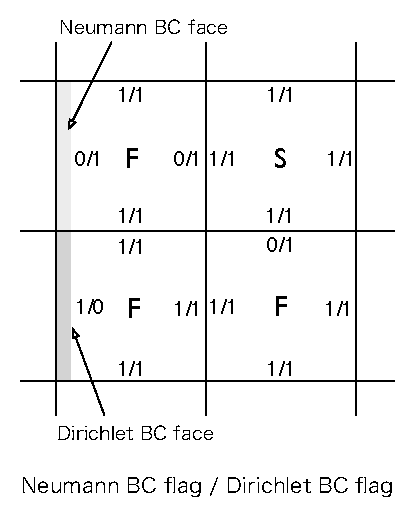
\includegraphics[width=5.5cm,clip]{bit_flag_P.eps}
\end{center}
\caption{圧力反復式に用いるビットフラグ.各セルについて,6つのフラグ(三次元の場合)を設定する.Sセルは固体セル,Fセルは通常の流体セルであり,この例では,左下のセルにDirichlet境界,左上のセルにNeumann境界が与えられている.Neumann BCフラグは,Neumann条件が与えられたセル面と固体セルに接する流体セルの接触面をゼロに設定する.}
\label{fig:N&D bit flag}
\end{figure}


%
\paragraph{連立一次方程式の係数行列と定数ベクトルの計算}
\textbf{式(\ref{eq:ebcs_poisson3})}を離散化して得られる連立一次方程式$\mathrm{A}\,\bm{x}=\bm{b}$の係数行列$\mathrm{A}$と定数ベクトル$\bm{b}$については,前述したポリシーから以下のようにまとめられる.

\begin{itemize}
\item ビットフラグの計算\\
エンコードして保持しておくフラグは,次の4種類である.
\begin{equation}
\small
\left.
\begin{array}{lll}
\vspace{2mm}
\displaystyle{ \phi^{\,D}_{\,l}\, \phi^{\,N}_{\,l} } & 6方向\,\times\,1\,\mathrm{bit}\quad (6\,\mathrm{bits}) & \mathrm{ BC\_NDAG\_\{E,W,N,S,T,B\} } \\
\vspace{2mm}
\displaystyle{ \phi^{\,N}_{\,l} } & 6方向\,\times\,1\,\mathrm{bit}\quad (6\,\mathrm{bits}) & \mathrm{ BC\_N\_\{E,W,N,S,T,B\} }\\
\vspace{2mm}
\displaystyle{ \phi^{\,D}_{\,l} } & 6方向\,\times\,1\,\mathrm{bit}\quad (6\,\mathrm{bits}) & \mathrm{ BC\_D\_\{E,W,N,S,T,B\} }\\
\vspace{2mm}
\displaystyle{ \sum \limits_l \left( \, \phi^{\,N}_{\,l} \, \right) } & 1 \sim 6 \quad (3\,\mathrm{bits}) & \mathrm{ BC\_DIAG }\\
\end{array} \quad \right\}
\label{eq:bit flag}
\end{equation}

\item 定数ベクトルの計算\\
計算内部領域における固体セルを計算する場合,定数項を$\psi=0$と修正する.
\end{itemize}

%
\paragraph{圧力Poisson部の計算手順}
\textbf{式(\ref{eq:ebcs_poisson3})}を\textbf{\ref{eq:poisson_iteration}}の手順で解く場合,ソース項の処理は以下のように考える.

\begin{indentation}{3zw}{0zw}
{ \small
\noindent begin: Time step loop\\
\hspace{1cm}pseudo vectorの計算\\
\hspace{1cm}Poissonのソース項 $\gamma^{\,0}$の計算\\
\hspace{1cm}Poissonのソース項 $\gamma^{\,N1}$の計算(反復中に変化しない条件:壁面,対称,流出)\\
\hspace{1cm}Poissonのソース項 $\gamma^{\,D}$の計算(流出,遠方,流入出)\\
\hspace{1cm}begin: Iteration loop\\
\hspace{2cm}Poissonのソース項 $\gamma^{\,N2}$の計算(反復中に変化する条件:壁面,流入)\\
\hspace{2cm}Poissonの求解(\textbf{式\ref{eq:poisson_iteration}})\\
\hspace{1cm}end: Iteration loop\\
end: Time step loop\\
}
\end{indentation}

反復中に変化するNeumann条件は,壁面境界で圧力勾配をNavier-Stokes方程式から求める場合と流入境界の場合である.ソース項の計算タイミングとして,圧力Poissonの反復前と反復内の2通りがある.$\gamma^{\,N1}$は反復前に決まる条件である.一方,壁面境界や流入境界でNS式から圧力勾配を計算する$\gamma^{\,N2}$は反復内で処理する.したがって,ソース項は2つの配列を使って実装している.

\end{indentation}

%
\subsubsection{Fractional Step法における射影ステップの処理}
コロケート変数配置のFractional Step法の計算処理では,セルセンタとセルフェイスに配置された速度ベクトルに対して,\textbf{式(\ref{eq:Pressure correction CC}}, \textbf{\ref{eq:Pressure correction CF})}に示すそれぞれ圧力勾配による射影ステップの計算が必要になる.再掲すると,

\begin{equation}
\left.
\begin{array}{llll}
u_i^{\,n+1} &=& \displaystyle{ u_i^{\,*} - \Delta t {\frac{\partial p}{\partial x_i}}^{n+1} } & \mathrm{(Cell\,center)} \vspace{2mm}\\
u_{i,\,face}^{\,n+1} &=& \displaystyle{ \bar{u}_{i,\,face}^{\,*} - \Delta t {\frac{\partial p}{\partial x_i}}^{n+1} } & \mathrm{(Cell\,face)}\\
\end{array} \qquad \right \}
\label{eq:prj step}
\end{equation}

\textbf{式(\ref{eq:prj step})}の圧力勾配項に対して,\textbf{式(\ref{eq:ebcs_dirichlet})}の圧力勾配の離散式を適用する.

%
\paragraph{セルセンタの圧力勾配}
x方向を例にして,セルセンタの場合の圧力勾配の離散化を示す.

\begin{equation}
\begin{array}{lll}
{\nabla p}_{c,\,x} &=& \displaystyle{ \frac{1}{2} \left( {\nabla p}_e + {\nabla p}_w \right) } \vspace{2mm}\\
 &=& \displaystyle{ \frac{1}{2} \left[
 {\left( \nabla p\,\phi^{\,N} \right)}_e + \left( 1-\phi^{\,N}_e \right) \nabla p^{BC}_e
+{\left( \nabla p\,\phi^{\,N} \right)}_w + \left( 1-\phi^{\,N}_w \right) \nabla p^{BC}_w
 \right] } \vspace{2mm}\\
 &=& \displaystyle{ \frac{1}{2} \left[ \frac{1}{h} \left\{ \phi^{\,D}_e p_{i+1} + \left( 1-\phi^{\,D}_e \right) p^{BC}_{i+1} -p_i \right\} \phi^{\,N}_e + \left( 1-\phi^{\,N}_e \right) \nabla p^{BC}_e \right.} \vspace{2mm}\\
 & & \displaystyle{ \left. + \frac{1}{h} \left\{ p_i - \phi^{\,D}_w p_{i-1} - \left( 1-\phi^{\,D}_w \right) p^{BC}_{i-1} \right\} \phi^{\,N}_w + \left( 1-\phi^{\,N}_w \right) \nabla p^{BC}_w \right]} \vspace{2mm}\\
 &=& \displaystyle{ \underbrace{ \frac{1}{2h} \left\{ \phi^{\,D}_e \phi^{\,N}_e p_{i+1} + \left( \phi^{\,N}_w - \phi^{\,N}_e \right) p_i - \phi^{\,D}_w \phi^{\,N}_w p_{i-1} \right\} }_{(i)} } \vspace{2mm}\\
 & & \displaystyle{ + \underbrace{ \frac{1}{2} \left[
 \frac{1}{h} \left\{ \left( 1-\phi^{\,D}_e \right) \phi^{\,N}_e p^{BC}_{i+1} 
 - \left( 1-\phi^{\,D}_w \right) \phi^{\,N}_w p^{BC}_{i-1} \right\} 
 + \left( 1-\phi^{\,N}_e \right) \nabla p^{BC}_e + \left( 1-\phi^{\,N}_w \right) \nabla p^{BC}_w
 \right] }_{(ii)} } \vspace{2mm}\\
\end{array}
\label{eq:grad p CC}
\end{equation}

\textbf{式(\ref{eq:grad p CC})}において,(i)の項は非境界条件部分の圧力勾配を示す.一方,(ii)の項はDirichlet条件とNeumann条件による圧力勾配を示し,反復ループ外で設定する.
ガイドセルに接しない内部領域は$\nabla p=0$の条件のみなので,(ii)項はゼロとしてよい.
ガイドセルに接する内部領域では,外部境界条件OUTFLOW, TRACTION\_FREEにより$p=0$のDirichlet条件が課せられる場合がある.その場合も参照値がゼロなので,(ii)の評価は不要になる.
$\nabla p=0$の条件を考慮して,\textbf{式(\ref{eq:grad p CC})}を簡潔に表記すると,

\begin{equation}
\begin{array}{lll}
{\nabla p}_{c,\,x}  &=& 
\displaystyle{ \frac{1}{2h} \left\{ \phi^{\,D}_e \phi^{\,N}_e p_{i+1} + \left( \phi^{\,N}_w - \phi^{\,N}_e \right) p_i - \phi^{\,D}_w \phi^{\,N}_w p_{i-1} \right\} }\\
\end{array}
\label{eq:grad p CC 2}
\end{equation}

\paragraph{セルフェイスの圧力勾配}
次に,$i+1$セルがディリクレ境界の場合のセルフェイスの圧力勾配を示す.

\begin{equation}
\begin{array}{lll}
{\nabla p}_{i+1/2,\,x} &=& \displaystyle{ 
 {\left( \nabla p\,\phi^{\,N} \right)}_{i+1/2} + \left( 1-\phi^{\,N}_{i+1/2} \right) \nabla p^{BC}_{i+1/2} } \vspace{2mm}\\
 &=& \displaystyle{ \frac{1}{h} \left\{ \phi^{\,D}_{i+1/2} \, p_{i+1} + \left( 1-\phi^{\,D}_{i+1/2} \right) p^{BC}_{i+1} -p_i \right\} \phi^{\,N}_{i+1/2} + \left( 1-\phi^{\,N}_{i+1/2} \right) \nabla p^{BC}_{i+1/2} } \vspace{2mm}\\
 &=& \displaystyle{ \underbrace{ \frac{1}{h} \left( \phi^{\,D}_{i+1/2} \, \phi^{\,N}_{i+1/2} \, p_{i+1} - \phi^{\,N}_{i+1/2} \, p_i \right) }_{(i)}
 + \underbrace{ \frac{1}{h} \left( 1-\phi^{\,D}_{i+1/2} \right) \phi^{\,N}_{i+1/2} \, p^{BC}_{i+1} 
 + \left( 1-\phi^{\,N}_{i+1/2} \right) \nabla p^{BC}_{i+1/2} }_{(ii)} }\\
\end{array}
\label{eq:grad p CF}
\end{equation}

\textbf{式(\ref{eq:grad p CF})}において,(i)の項は非境界条件部分の圧力勾配,(ii)は境界条件により指定される圧力勾配を示す.圧力勾配の境界条件によるセルフェイスにおける修正も,セルセンターの場合と同様に,領域境界上の圧力勾配がririchlet型で与えられる場合のみを考慮すればよい.
また,スタガード配置の境界上における速度ベクトルのインデクスは$i=0, imax$であり,$i=0$の場合には対応するビットフラグを設定する.$\nabla p=0,\,p=0$を考慮すると,

\begin{equation}
\begin{array}{llll}
X-面) & {\nabla p}_{1/2} &=& \displaystyle{ \frac{1}{h} \left( \phi^{\,N}_{1/2} \, p_1 - \phi^{\,D}_{1/2} \, \phi^{\,N}_{1/2} \, p_0 \right) } \vspace{2mm}\\
X+面) & {\nabla p}_{ix+1/2} &=& \displaystyle{ \frac{1}{h} \left( \phi^{\,D}_{i+1/2} \, \phi^{\,N}_{i+1/2} \, p_{ix+1} - \phi^{\,N}_{i+1/2} \, p_{ix} \right) } \vspace{2mm}\\
\end{array}
\label{eq:grad p CF 2}
\end{equation}

結局,ディリクレ型として$p=0$を考える限りにおいては,修正項は不要となる.

%%%
\subsection{対流項の扱い}
\hypertarget{tgt:convection term}{対流項の空間スキーム}は保存的な差分法により離散化する.つまり,有限体積法と同様にセル界面での数値流束を求め,発散型と親和性の高い流束ベースの評価を行う.

\subsubsection{MUSCL形式}
対流項スキームについて,一次元を例に示す.インデクス${}_i$はセルセンター位置を示し,ハーフインデクス${}_{i\pm1/2}$はセル界面を意味する.

対流項スキームには,セル内部の分布形を仮定し,分布を再構築して精度を上げるMUSCL\index{MUSCL}スキームを形式的に利用する~\cite{fujii:94:CFD}.分布形として線形 (piecewise linear) と放物形 (piecewise parabolic) の仮定はそれぞれ二次と三次の近似精度に相当する.Taylor展開から非移流物理量$\varphi$の分布を再構成すると,

\begin{equation}
\varphi(x) \,=\,
\varphi_i \,+\, 
\left( x-x_i \right) \frac{\varphi_{\,i+1} - \varphi_{\,i-1}}{2\Delta x} \,+\, 
\frac{3\kappa}{2} \left[ {\left( x-x_i \right)}^2
\,-\, \frac{{(\Delta x)}^2}{12} \right] \frac{\varphi_{i+1} - 2\varphi_i + \varphi_{i-1}}{{(\Delta x)}^2}
\quad \left( \, x_{i-1/2} \, \leq \,x\, \leq \, x_{i+1/2} \, \right)
\label{eq:reconstruction}
\end{equation}

\noindent セル境界における左右(L, R)の物理量は,
\begin{equation}
\left.
\begin{array}{llll}
\vspace{2mm}
{\left( \varphi_R \right)}_{\,i+1/2} &=& \varphi_{\,i+1} & \displaystyle{ - \, \frac{\varepsilon}{4} \left[ \, \left( 1 \,-\, \kappa \right) \Delta_{\,i+1\,} \varphi \,+\, \left( 1+\kappa \right) \Delta_{\,i\,} \varphi \,\right] } \\
\vspace{2mm}
{\left( \varphi_L \right)}_{\,i+1/2} &=& \varphi_{\,i} & \displaystyle{ + \, \frac{\varepsilon}{4} \left[ \, \left( 1 \,-\, \kappa \right) \Delta_{\,i-1\,} \varphi \,+\, \left( 1 \,+\, \kappa \right) \Delta_{\,i\,} \varphi \,\right] } \\
\vspace{1mm}
& & & \Delta_{\,i\,} \varphi \,=\, \varphi_{\,i+1} - \varphi_{\,i} \\
\end{array} \quad \right\}
\label{eq:MUSCLE interpolation}
\end{equation}

\noindent となる.$\varepsilon$は精度を切り替えるパラメータで$\kappa$は分布形を制御する.

\begin{equation}
\varepsilon \,=\, \left\{
\begin{array}{cl}
\vspace{1mm}
0 & \mathrm{1st\, order\, upwind} \\
\vspace{1mm}
1 & \mathrm{Higher\, order} \\
\end{array} \right.
\label{eq:MUSCL parameter1}
\end{equation}

\begin{equation}
\kappa \,=\, \left\{
\begin{array}{cl}
\vspace{1mm}
1   & \mathrm{2nd\, order\,central} \\
\vspace{1mm}
1/3 & \mathrm{3rd\, order\,upwind} \\
\end{array} \right.
\label{eq:MUSCL parameter2}
\end{equation}

\noindent 上記により求められたセル界面の両側の物理量の値を用いて,数値流束を計算する.ALE形式を考慮して移流速度を$u-u^{\,g}$,非移流物理量を$\varphi$とすると,物理流束は次式となる.

\begin{equation}
f \,=\, \left( u - u^{\,g} \right) \varphi
\label{eq:physical flux ALE}
\end{equation}

\noindent セル界面${}_{i\pm1/2}$における数値流束$\tilde{f}_{\,i\pm1/2}$は次式で表せる.

\begin{equation}
\tilde{f}_{\,i\pm1/2} \,=\,
\frac{1}{2} { \left[ \, \left( f_R + f_L \right) \,-\, \left| (u-u^{\,g}) \right| \left( \varphi_R - \varphi_L \right) \, \right] }_{\,i\pm1/2}
\label{eq:general flux form}
\end{equation}

%
\subsubsection{minmodリミター}
MUSCLスキームのリミターは,主に圧縮性で衝撃波が生じるような不連続を扱う場合に,単調性を維持し,TVD安定性を確保するために導入される.
ここではminmod limiterについて示す.
minmod limiterは次式で表される勾配制限関数である.

\begin{equation}
\mathrm{minmod}(x,y) \,=\, \mathrm{sgn}(x) \, \mathrm{max}[0,\,\mathrm{min}\{ |x|,\, \mathrm{sgn}(x)y\} ]
\label{eq:minmod limiter}
\end{equation}

いま,$i$セルの両側のセル界面における数値流束を考える.
\textbf{図\ref{fig:muscl_stencil}}を参照して,\textbf{式(\ref{eq:MUSCLE interpolation})}にminmod limiterを適用すると,

\begin{equation}
\left.
\begin{array}{llll}
\vspace{1mm}
(\varphi_R)_{\,i+1/2} & = & \varphi_{\,i+1} & \displaystyle{ - \, \frac{\varepsilon}{4} \left[ \, (1-\kappa) \overline{\Delta^+}  \,+\, (1+\kappa) \overline{\Delta^-}\,\right]_{\,i+1} } \\
\vspace{1mm}
(\varphi_L)_{\,i+1/2} & = & \varphi_{\,i} & \displaystyle{ + \, \frac{\varepsilon}{4} \left[ \, (1-\kappa) \overline{\Delta^-}  \,+\, (1+\kappa) \overline{\Delta^+}\,\right]_{\,i} } \\
\vspace{1mm}
(\varphi_R)_{\,i-1/2} & = & \varphi_{\,i} & \displaystyle{ - \, \frac{\varepsilon}{4} \left[ \, (1-\kappa) \overline{\Delta^+}  \,+\, (1+\kappa) \overline{\Delta^-}\,\right]_{\,i} } \\
\vspace{1mm}
(\varphi_L)_{\,i-1/2} & = & \varphi_{\,i-1} & \displaystyle{ + \, \frac{\varepsilon}{4} \left[ \, (1-\kappa) \overline{\Delta^-}  \,+\, (1+\kappa) \overline{\Delta^+}\,\right]_{\,i-1} } \\
\end{array} \qquad \right\}
\label{eq:MUSCL minmod}
\end{equation}

\noindent ここで,

\[
\left.
\begin{array}{lll}
\vspace{1mm}
\Delta^+_i & = & \varphi_{\,i+1} - \varphi_{\,i}\\
\vspace{1mm}
\Delta^-_i & = & \varphi_{\,i} - \varphi_{\,i-1}\\ 
\end{array}
\qquad \right\} \qquad \equiv d_{\,(1,\,2,\,3,\,4)}
\]

\[
\left.
\begin{array}{lll}
\vspace{1mm}
\overline{\Delta^+_i} & = & \mathrm{minmod} ( \Delta^+_i, \,b\Delta^-_i )\\
\vspace{1mm}
\overline{\Delta^-_i} & = & \mathrm{minmod} ( \Delta^-_i, \,b\Delta^+_i )\\ 
\end{array}
\qquad \right\}
\]

\[
\hspace{1cm} b = \frac{3-\kappa}{1-\kappa}
\]

\noindent である.

\begin{figure}[htbp]
\begin{center}
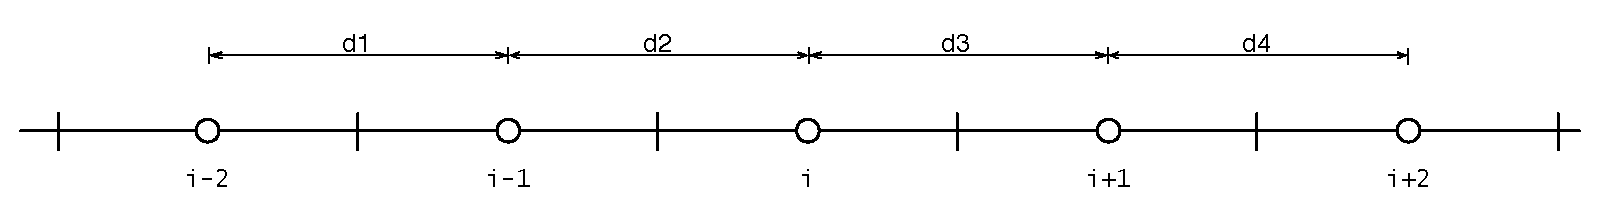
\includegraphics[width=15cm,clip]{muscl_stencil.eps}
\end{center}
\caption{MUSCLスキームのステンシル.d1,d2,d3,d4はセルセンタで定義される物理量の区間で,セル界面位置の速度の符号をs1,s2,s3,s4とする.}
\label{fig:muscl_stencil}
\end{figure}

コード中の実装は次の通り.
\[
\begin{array}{llll}
\vspace{1mm}
\mathrm{g6}; & \overline{\Delta^+_{i+1}} & = \mathrm{minmod}(\Delta^+_{i+1},\,b\Delta^-_{i+1}) & = \mathrm{s4} \cdot \mathrm{max}[0,\,\mathrm{min}\{ |\mathrm{d4}|,\, \mathrm{s4\,b\,d3}\} ] \\
\vspace{1mm}
\mathrm{g5}; & \overline{\Delta^-_{i+1}} & = \mathrm{minmod}(\Delta^-_{i+1},\,b\Delta^+_{i+1}) & = \mathrm{s3} \cdot \mathrm{max}[0,\,\mathrm{min}\{ |\mathrm{d3}|,\, \mathrm{s3\,b\,d4}\} ] \\
\vspace{1mm}
\mathrm{g4}; & \overline{\Delta^+_{i}} & = \mathrm{minmod}(\Delta^+_{i},\,b\Delta^-_{i}) & = \mathrm{s3} \cdot \mathrm{max}[0,\,\mathrm{min}\{ |\mathrm{d3}|,\, \mathrm{s3\,b\,d2}\} ] \\
\vspace{1mm}
\mathrm{g3}; & \overline{\Delta^-_{i}} & = \mathrm{minmod}(\Delta^-_{i},\,b\Delta^+_{i}) & = \mathrm{s2} \cdot \mathrm{max}[0,\,\mathrm{min}\{ |\mathrm{d2}|,\, \mathrm{s2\,b\,d3}\} ] \\
\vspace{1mm}
\mathrm{g2}; & \overline{\Delta^+_{i-1}} & = \mathrm{minmod}(\Delta^+_{i-1},\,b\Delta^-_{i-1}) & = \mathrm{s2} \cdot \mathrm{max}[0,\,\mathrm{min}\{ |\mathrm{d2}|,\, \mathrm{s2\,b\,d1}\} ] \\
\vspace{1mm}
\mathrm{g1}; & \overline{\Delta^-_{i-1}} & = \mathrm{minmod}(\Delta^-_{i-1},\,b\Delta^+_{i-1}) & = \mathrm{s1} \cdot \mathrm{max}[0,\,\mathrm{min}\{ |\mathrm{d1}|,\, \mathrm{s1\,b\,d2}\} ] \\
\end{array}
\]

%
\subsubsection{バイナリボクセルの場合の固体壁面境界処理}
バイナリボクセルによる物体形状表現では,計算空間内の任意のセルが物体(非流体)セルになる.対流項スキームの近似精度が高くなるとステンシルが広がり,参照セルが非流体セルのときの処理を適切に行わなくてはならない.

物理流束は\textbf{式(\ref{eq:physical flux ALE})}で表せるので,セルの6面について和をとると,対流項は次のように離散化される.

\begin{equation}
\frac{\partial f}{\partial x_j} \, \equiv \, \frac{1}{h} \sum  \limits_l \tilde{f}_l \,n_l 
\,=\, \frac{1}{h} \sum  \limits_l 
\frac{1}{2} { \left[ \, \left( f_R + f_L \right) \,-\, \left| (u-u^{\,g}) \right| \left( \varphi_R - \varphi_L \right) \, \right] }_{\,l} \, n_l
\label{eq:upwind approx}
\end{equation}

\noindent ここで$n_l$はセルの各面における外側法線であり,移流速度は各面に垂直な方向成分と考える.

バイナリボクセルでは,セルの状態を表すマスク関数$\phi$により形状を階段状に近似する.$\phi$は\textbf{式(\ref{eq:mask function})}として定義され,このマスク関数を用いて界面位置を調べ\footnote{事前に各セルの状態について,ビットフラグ(STATE\_BIT)にエンコードしておく.計算時には,デコードしたフラグから\textbf{式(\ref{eq:mask at cell face})}と式(\ref{eq:wall vel at cell face})を評価する.対流項部分の計算は演算量が多く,if文の分岐でも速度低下は小さいことを確認している(Intel Compiler 11.1).},壁面境界条件をスキーム中に取り込む\cite{akasaka:06:JSCES}.
\textbf{図\ref{fig:Mask pattern CC}}のようなコロケート配置におけるセルの状態パターンに対して,セルiでの計算を考える.

\begin{figure}[htbp]
\begin{center}
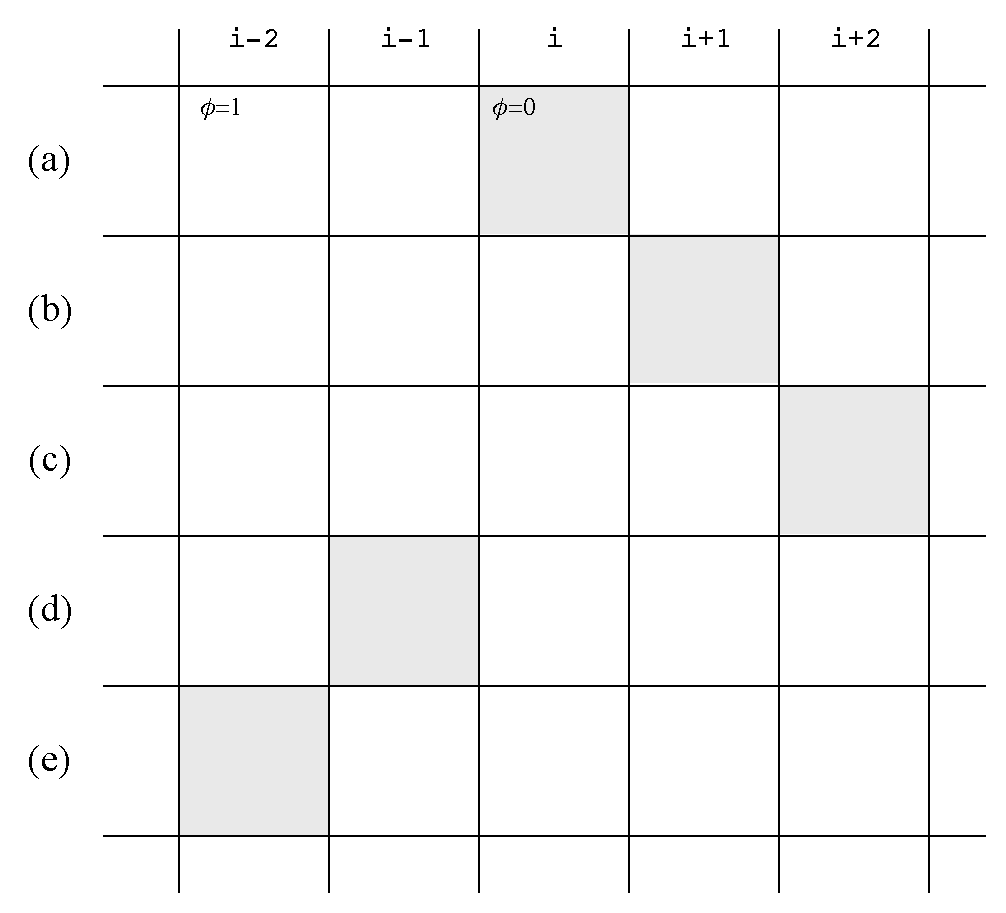
\includegraphics[width=8cm,clip]{mask_patternCC.eps}
\end{center}
\caption{対流項の計算で考慮するマスクパターン.網掛けの部分は非流体セル$\phi=0$,それ以外は流体セル$\phi=1$を示す.(a)$\sim$(e)のパターンは横方向に一次元的な分布を表している.}
\label{fig:Mask pattern CC}
\end{figure}

\begin{enumerate}
\item (a)の場合は,セルiの計算結果自体がマスクにより無効となるので考慮する必要はない.
\item ステンシルが$i\pm2$である(b)$\sim$(e)の場合は,参照値を修正する.
\item (b), (d)のパターン,つまり参照する$i\pm1$セルが固体の場合にも参照値を修正する.更に,$i\pm1/2$位置の流束は,固定壁面があるので$\tilde{f}=0$となる.次式のように界面のフラグによりマスクし,流束をゼロにするように実装している.
\begin{equation}
\phi_{\,i\pm1/2} \,=\, \phi_{i} \times \phi_{i\pm1} \,=\, \left\{
\begin{array}{ll}
0 & \mathrm{Wall\, boundary\, face}\\
1 & \mathrm{Fluid\, face}\\
\end{array} \right.
\label{eq:mask at cell face}
\end{equation}

\begin{equation}
\tilde{f}_{i\pm1/2} \,=\, \phi_{\,i\pm1/2} \, \tilde{f}_{i\pm1/2}
\label{eq:wall vel at cell face}
\end{equation}
\noindent ここで右辺の$\tilde{f}_{i\pm1/2}$は\textbf{式(\ref{eq:general flux form})}の評価式である.
\end{enumerate}

%
\subsubsection{参照値の修正}
\textbf{図\ref{fig:Mask pattern CC}}の各パターンに対して,対象セルの対流項を計算する場合の参照値の修正について考える.バイナリボクセルの形状表現では,物体境界は必ずセル界面にある.どのセル界面が固体境界面であるかは,セルの状態$\phi$を見て判断し,固体境界面における参照値は流体セル側からの線形分布を仮定する.パターン(b), (d)の場合,参照値$\varphi_{\,i\pm1}$を次のように近似する.$\varphi_{\,i\pm1/2\, face}$は境界値として与えられるものとする.

\begin{equation}
\varphi_{\,i\pm1} \,=\, 2 \,\varphi_{\,i\pm1/2\, face} - \varphi_{\,i}
\label{eq:solid face reference 1}
\end{equation}

\noindent 同様に,$\varphi_{\,i\pm2}$が参照値となる(c), (e)の場合についても$\varphi_{\,i\pm3/2\, face}$を境界値として与え,次式で修正する.

\begin{equation}
\varphi_{\,i\pm2} \,=\, 2 \,\varphi_{\,i\pm3/2\, face} - \varphi_{\,i\pm1}
\label{eq:solid face reference 2}
\end{equation}

%
\subsection{粘性項の扱い}
粘性項は,非圧縮条件を用いて簡略化して扱う.

\begin{equation}
\frac{1}{Re} \frac{\partial}{\partial x_j} \left( \frac{\partial u_i}{\partial x_j} + \frac{\partial u_j}{\partial x_i} \right)
\,=\, \frac{1}{Re} \frac{\partial}{\partial x_j} \left( \frac{\partial u_i}{\partial x_j} \right) 
\label{eq:viscous incomp approx}
\end{equation}

\noindent 対流項と同様に参照値の修正を行い,評価する.ベクトル成分$\varphi$について,Euler陽解法の場合について\textbf{式(\ref{eq:viscous approx})}に示す.

\begin{equation}
\frac{1}{Re} \frac{\partial}{\partial x_j} \left( \frac{\partial \varphi}{\partial x_j} \right)
\,\approx\, \frac{1}{Re\,h^2} \left\{\, \sum \limits_l \left( \varphi_{\,l} \right) \,-\, 6 \,\varphi_{\,i,j,k} \right\}
\label{eq:viscous approx}
\end{equation}

\noindent $\sum \limits_l \left( \varphi_{\,l} \right)$は,対象セルの隣接6セルの$\varphi$の和を意味する.


%
\subsection{境界条件処理}
\textbf{\ref{sec:fractional step}}のFractional Step法の手順では,疑似速度ベクトルを求めるプロセスで対流項と粘性項の計算を行い,その後境界条件処理を行う.
境界条件には,外部境界条件と計算領域内部で用いる境界条件の2種類が設定できる.
CBCソルバークラスで指定できる速度の境界条件を\textbf{表\ref{tbl:BCs of velocity}}に示す.

\begin{table}[htdp]
\small
\caption{計算領域内部と外部境界に指定できる速度境界条件の種類}
\begin{center}
\begin{tabular}{l|cc|ll} \toprule
境界条件の種類 & 内部 & 外部 & 外部境界の実装方式 & コメント\\ \midrule
壁面境界 & ○ & ○ & 流束形式 & フラグによりスキーム中に組み込まれている\\
対称境界 & - & ○ & 境界値指定 &\\
流入境界 & ○ & ○ & 流束形式 & Dirichlet型による速度指定(一定値と単振動条件)\\
流出境界 & ○ & ○ & 流束形式 & 対流流出,内部境界は面直のみ\\
遠方境界 & - & ○ & 境界値指定 & トラクションフリー\\
流入出境界 & - & ○ &  & 流出境界と,(流入として)遠方境界の切り替え\\
周期境界 & - & ○ & 境界値指定 & データコピー\\ \bottomrule
\end{tabular}
\end{center}
\label{tbl:BCs of velocity}
\end{table}

%
\subsubsection{速度境界条件のビットフラグ}
速度境界条件を認識するために,圧力の場合と同様にビットフラグを導入する.\textbf{図\ref{fig:bit flag V}}に示すように,各セルの6面についてフラグがセットされる.このフラグは各面に割り当てられた境界条件の識別子を示す.具体的には,媒質と境界条件の属性リストであるコンポーネントの登録番号である.CBCの実装では,コンポーネントは媒質と境界条件の個数を合わせて30個まで保持できる.各面に5ビット幅を割り当て,値の0は不使用(つまり,境界条件なし),31は外部境界の認識に利用している($2^5-2$個).\footnote{コンポーネント個数はParseBC::setControlVars()でチェック.}.\textbf{表\ref{tbl:Flags in bcv}}に具体的なビット割り当てを示す.

\begin{figure}[htbp]
\begin{center}
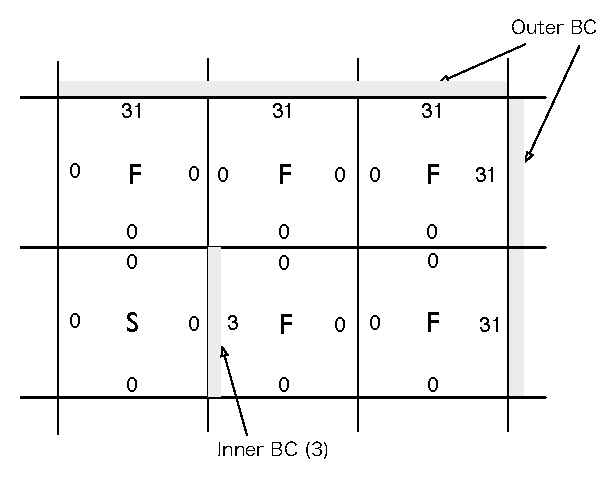
\includegraphics[width=8cm,clip]{bit_flag_V.eps}
\end{center}
\caption{速度境界条件に用いるビットフラグ.各セルについて,6つのフラグ(三次元の場合)を設定する.Sセルは固体セル,Fセルは通常の流体セルである.この例では内部境界条件として,コンポーネントの登録番号3の境界条件がひとつ指定されている.外部境界には,認識番号31が登録される.}
\label{fig:bit flag V}
\end{figure}

%
\subsubsection{内部境界条件}
固体壁条件については,計算空間内に任意の箇所に現れる可能性があるため,前述したようにフラグを用いて壁面の影響を流束形式によりスキームに導入する.
一方,流入と流出条件は,その処理は煩雑で効率的な実装が難しい場合が多いので,演算速度はあまり期待できない.しかしながら,指定する速度境界条件は一般的に局所的になる傾向があるため,境界条件処理かどうかを探索する範囲をバウンディングボックスで絞り込んでおくことにより,演算処理自体を少なくできる.
このため,コンポーネント単位で処理を行う.
境界条件の導入は,圧力の場合の\textbf{式(\ref{eq:ebcs_flagging})}と同様に,境界マスクと流束を次式により評価する.

\begin{equation}
\phi^{\,BC} \,=\, \left\{
\begin{array}{ll}
0 & \mathrm{Face\, that\, boundary\, condition\, is\, given}\\
1 & \mathrm{Normal\, face}\\
\end{array} \right.
\label{eq:mask function velocity}
\end{equation}

\begin{equation}
\tilde{f}_{i\pm1/2} \,=\, \phi^{\,BC} \tilde{f}_{i\pm1/2} \,+\, \left( 1-\phi^{\,BC} \right)\, \tilde{f}_{i\pm1/2}^{\,BC}
\label{eq:ebcs_flagging_vel}
\end{equation}

\noindent 実装としては,\textbf{式(\ref{eq:ebcs_flagging_vel})}を2パスで構成する.つまり,最初のループで固体壁の影響を考慮した流束$\tilde{f}_{i\pm1/2}$を計算し,境界条件が指定された面の流束は計算しない.次のループで,境界条件面のみ流束$\tilde{f}^{\,BC}_{i\pm1/2}$を計算し,寄与分を加算する.
内部境界条件は,ひとかたまりで格子線に沿って面直な流入・流出面をもつものを想定している.これらの境界条件は,流束形式でスキーム中に取り込まれる.また,補助的にセルフェイス位置の速度にも境界条件を与える.

%
\subsubsection{外部境界条件}
外部境界条件の実装には,2種類の方法を用いている.一つは,内部境界と同じく空間項の評価時に境界部分の流束を評価する方法である.もう一つは,一般的に行われている値を代入する方法である.後者の方法は,代入すべき位置(セル)が存在し,一意に決まる値で参照のみが行われる場合に用いる.

壁面境界は,空間項の評価時に壁面位置を感知し,その影響を境界条件として取り込む離散化を行っているので,特別な処理を必要としない.ただし,前処理として,指定された境界面に対して固体のIDをガイドセル部分に付与しておく.

流入と流出境界は,内部境界と同様な実装をで,処理単位は各面毎としている.

対称条件,遠方条件,周期条件については,境界値を指定する.


\pagebreak
%%%
\section{距離情報を用いた形状近似の解法}
形状の近似として,物理量の定義点から物体までの\hypertarget{tgt:dist_info_scheme}{距離情報のみを用いた形状近似}を考える.
前処理時の入力情報としてSTLなどの形状データを考え,含まれる三角形要素と格子の交点情報を計算する.
これより,距離情報が得られる.
この場合,入力のSTLが完全に形状を表現できていなくても,STLとして三角形要素が定義できていれば交点情報が必ず得られる.
また,定義点間に複数の交点があってもよい.
したがって,データフォーマットとして有効であれば,形状を完全に再現できていなくても,薄い物体でも扱うことが可能な利点がある.

%%
\subsection{実装の基本的な考え方}
コロケート格子における有限体積法ベースの流束計算に基づいて計算する.
物体近傍付近では,流束を構築する際に必要な速度の参照点の値を流体側から外挿することにより,物体の影響を考慮した流束を計算する.
したがって,物体の影響は全てセル界面の数値流束の近似に集約され,レギュラーのステンシルでの計算となる.

\textbf{図\ref{fig:distance stencil}}を参照して,セル$i$を積分する場合の壁面の影響をみる.
セル界面$i+1/2$側を考えると,次の2つの場合に分けられる.

\[
\begin{array}{lll}
\vspace{1mm}
(a) & 1/2 < d_i^+ < 1  & \varphi_{\,i+1/2}が定義でき,\tilde{f}_{\,i+1/2}が値をもつ. \\
\vspace{1mm}
(b) &  0 \le d_i^+ \le 1/2 & セル界面位置が固体内であるので\varphi_{\,i+1/2}が定義できない.\\  
\end{array}
\]

\begin{figure}[htbp]
\begin{center}
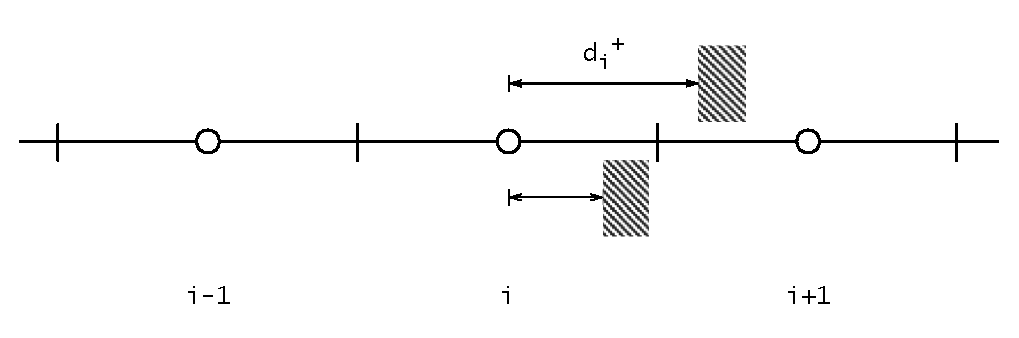
\includegraphics[width=10cm,clip]{distance_stencil.eps}
\end{center}
\caption{セル$i$を積分する場合の壁位置による影響.$d$は格子幅で正規化された無次元距離を表す.}
\label{fig:distance stencil}
\end{figure}

\noindent $d_i^{\pm}$は格子幅で正規化された距離で,$i$点における正負方向の距離を表し,[0,1]の値をとる.
$\varphi$は物理量で,例えば速度である.

(b)の場合には,セル界面位置が固体壁内部に位置するので,取り扱いを検討する.方法として,$\tilde{f}_{\,i+1/2}=0$と考えるやり方と,以下のように参照点の値を修正してそのまま計算するやり方が考えられる.とりあえず,後者を選択.
したがって,(a)の場合のみについて流束計算を考える.

参照点の外挿は,\textbf{図\ref{fig:stable extrapolation}}のように$d_i^+\rightarrow0$となっても破綻しないように次式を用いる~\cite{akasaka:10:JSME}.

\begin{equation}
\varphi_{\,i+1} \,=\, \frac{1}{1/2+d_i^+} \left[ \frac{3}{2}\varphi_{\,I} - (1-d_i^+)\,\varphi_{\,i-1/2} \right]
\label{eq:stable extrapolation}
\end{equation}

\noindent 同様に,界面$i-1/2$の場合には,
\begin{equation}
\varphi_{\,i-1} \,=\, \frac{1}{1/2+d_i^-} \left[ \frac{3}{2}\varphi_{\,I} - (1-d_i^-)\,\varphi_{\,i+1/2} \right]
\label{eq:stable extrapolation-}
\end{equation}

\noindent ここで$\varphi_I$は壁面の値で指定値である.また,$\varphi_{\,i\pm1/2}$の値は,定義されていなければ内挿する.

\begin{figure}[htbp]
\begin{center}
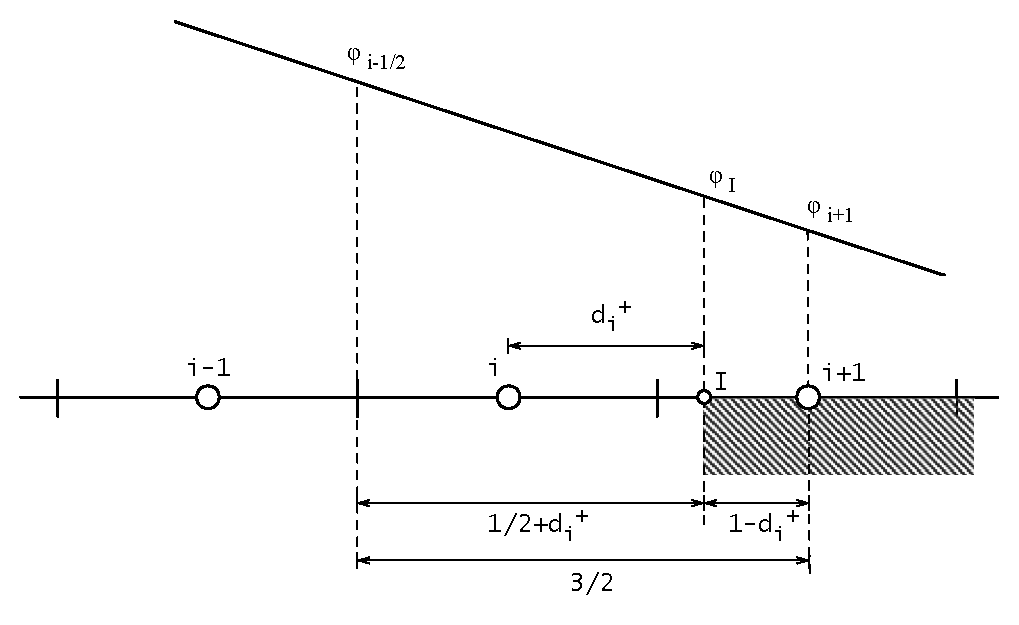
\includegraphics[width=11cm,clip]{extrapolation_stable.eps}
\end{center}
\caption{$(i+1)$セルが固体内にある場合の参照値$\varphi_{\,i+1}$の外挿.距離は格子幅$\Delta x$により正規化している.}
\label{fig:stable extrapolation}
\end{figure}

あるいは,少々不安定な実装として,次も考慮.
\begin{equation}
\displaystyle{ \varphi_{\,i\pm1} \,=\, \frac{1}{d_i^{\pm}} \left[ \varphi_{\,I} - \left( 1 - d_i^{\pm} \right) \varphi_{\,i} \right] }
\label{eq:unstable}
\end{equation}


%%
\subsection{距離情報を用いたMUSCLスキームの実装}
セル$i$に関する流束計算を高次精度のスキームを用いるとステンシルが広がる.
参照点間にカットが入るパターンに分類して,スキームの実装を述べる.

%
\subsubsection{対流項スキーム実装の詳細}
%まず,正負の各方向で$0 \le d_i^{\pm} \le 1/2 \, \mapsto \,\tilde{f}_{i\pm1/2}=0$とする.
%実装としては,次式のようにマスク関数$\chi$をかけて流束をゼロに強制する.

%\begin{equation}
%\tilde{f}_{\,i\pm1/2} \,=\,
%\frac{1}{2} { \left[ \, \left( f_R + f_L \right) \,-\, \left| (u-u^{\,g}) \right| \left( \varphi_R - \varphi_L \right) \, \right] }_{\,i\pm1/2} \, \chi
%\label{eq:masked flux form}
%\end{equation}

%\[
%\hspace{1cm}
%\chi \,=\,
%\left\{
%\begin{array}{ll}
%\vspace{1mm}
%0 & (0 \le d_i^{\pm} \le 1/2)\\
%\vspace{1mm}
%1 & (d_i^{\pm} > 1/2)\\
%\end{array}
%\right.
%\]

MUSCLスキームは片側3点の参照点をもつので,\hypertarget{tgt:modify by cut}{参照する物理量が壁面位置による修正}が必要かどうかを見ていく.

%
\paragraph{$\tilde{f}_{i-1/2}$の評価}
$\tilde{f}_{i-1/2}$を評価する場合,$u_{\,i-1/2}$の符号により参照するセルが異なる.
\[
\tilde{f}_{i-1/2}\,=\,
\left\{
\begin{array}{ll}
\vspace{1mm}
f(\varphi_{\,i-2},\,\varphi_{\,i-1},\,\varphi_{\,i}) & u_{\,i-1/2}\ge0\\
\vspace{1mm}
f(\varphi_{\,i-1},\,\varphi_{\,i},\,\varphi_{\,i+1}) & u_{\,i-1/2}<0\\
\end{array}
\right.
\]

壁面の影響による修正が必要な場合とは,参照する定義点間に交点が存在する場合である.
各セルで計算した距離情報の値を判定すれば,交点があるかどうかわかる.
つまり,$d\ne1$であれば交点が存在し,参照するセルの値を修正する必要がある.

%
\vspace{5mm}
\subparagraph{$u_{\,i-1/2}\ge0$の場合}
参照するセルは$(i-2,\,i-1,\,i)$であるが,$i$セルについての計算なので,修正対象となるセルは$(i-2,\,i-1)$セルである.

\begin{enumerate}
\item \textbf{図\ref{fig:stencil case 1}}に示すように,もし$d_i^- \ne 1$であれば,$(i-1)\sim (i)$間に交点が存在し,\textbf{式(\ref{eq:stable extrapolation-})}により$\varphi_{\,i-1}$の参照値を修正する.
\vspace{1mm}
\item 同じように,$d_{i-1}^- \ne 1$であれば,$\varphi_{\,i-2}$の修正が必要になる.
\begin{equation}
\varphi_{\,i-2} \,=\, \frac{1}{1/2+d_{i-1}^-} \left[ \frac{3}{2}\varphi_{\,I} - (1-d_{i-1}^-)\,\varphi_{\,i-1/2} \right]
\label{eq:modify i-2}
\end{equation}
\end{enumerate}

\begin{figure}[htbp]
\begin{center}
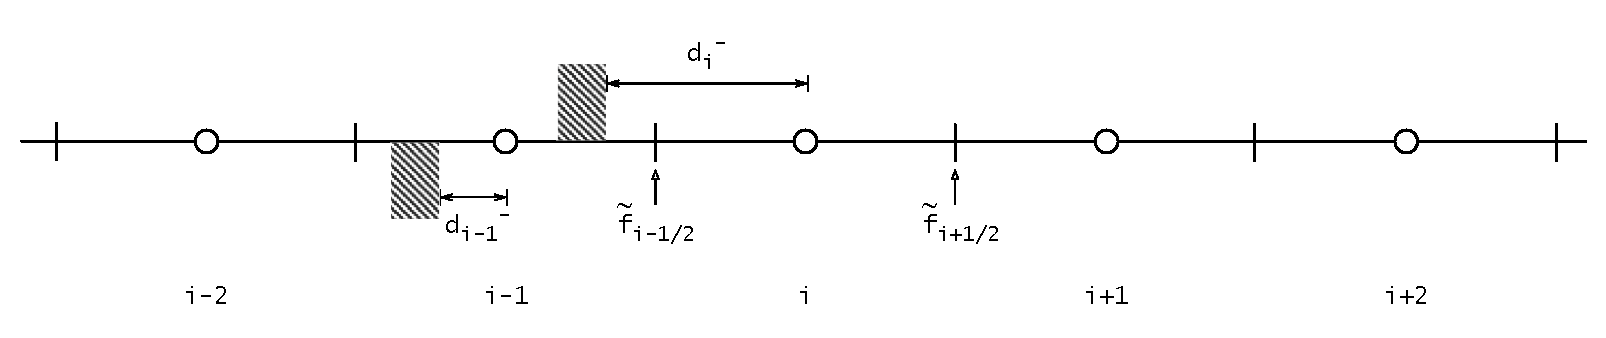
\includegraphics[width=15cm,clip]{stencil_case1.eps}
\end{center}
\caption{$\tilde{f}_{i-1/2}$評価時の$u_{\,i-1/2}\ge0$の場合の修正の判定.このときステンシルは$(i-2,\,i-1,\,i)$で,壁面の影響による修正を考慮する対象は$(i-2,\,i-1)$.}
\label{fig:stencil case 1}
\end{figure}


%
\vspace{5mm}
\subparagraph{$u_{\,i-1/2}<0$の場合}
参照するセルは$(i-1,\,i,\,i+1)$であるが,$i$セルについての計算なので,壁面が存在する場合の修正対象は$(i-1,\,i+1)$セルである.

\begin{enumerate}
\item \textbf{図\ref{fig:stencil case 2}}に示すように,もし$d_i^- \ne 1$であれば,$(i-1)\sim (i)$間に交点が存在し,\textbf{式(\ref{eq:stable extrapolation-})}により$\varphi_{\,i-1}$の参照値を修正する.
\vspace{1mm}
\item $d_{i}^+ \ne 1$であれば,\textbf{式(\ref{eq:stable extrapolation})}により$\varphi_{\,i+1}$を修正する.
\end{enumerate}

\begin{figure}[htbp]
\begin{center}
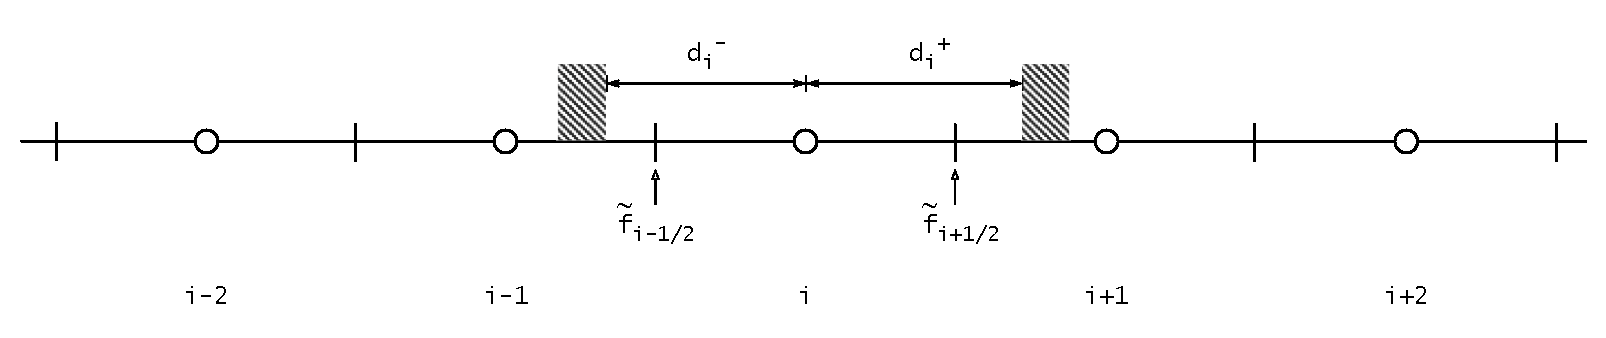
\includegraphics[width=15cm,clip]{stencil_case2.eps}
\end{center}
\caption{$\tilde{f}_{i-1/2}$評価時の$u_{\,i-1/2}<0$の場合,ステンシルは$(i-1,\,i,\,i+1)$で修正対象は$(i-1,\,i+1)$.$\tilde{f}_{i+1/2}$評価時の$u_{\,i+1/2}\ge0$の場合のステンシルも同様.}
\label{fig:stencil case 2}
\end{figure}


%
\paragraph{$\tilde{f}_{i+1/2}$の評価}
$\tilde{f}_{i+1/2}$を評価する場合,$u_{\,i+1/2}$の符号により参照するセルが異なる.
\[
\tilde{f}_{i+1/2}\,=\,
\left\{
\begin{array}{ll}
\vspace{1mm}
f(\varphi_{\,i-1},\,\varphi_{\,i},\,\varphi_{\,i+1}) & u_{\,i+1/2}\ge0\\
\vspace{1mm}
f(\varphi_{\,i},\,\varphi_{\,i+1},\,\varphi_{\,i+2}) & u_{\,i+1/2}<0\\
\end{array}
\right.
\]


%
\vspace{5mm}
\subparagraph{$u_{\,i+1/2}\ge0$の場合}
修正対象となるセルは$(i-1,\,i+1)$セルである.

\begin{enumerate}
\item \textbf{図\ref{fig:stencil case 2}}に示すように,もし$d_i^- \ne 1$であれば,$(i-1)\sim (i)$間に交点が存在し,\textbf{式(\ref{eq:stable extrapolation-})}により$\varphi_{\,i-1}$の参照値を修正する.
\vspace{1mm}
\item $d_{i}^+ \ne 1$であれば,\textbf{式(\ref{eq:stable extrapolation})}により$\varphi_{\,i+1}$を修正する.
\end{enumerate}


%
\vspace{5mm}
\subparagraph{$u_{\,i+1/2}<0$の場合}
修正対象となるセルは$(i+1,\,i+2)$セルである.

\begin{enumerate}
\item \textbf{図\ref{fig:stencil case 3}}に示すように,もし$d_i^+ \ne 1$であれば,\textbf{式(\ref{eq:stable extrapolation})}により$\varphi_{\,i+1}$の参照値を修正する.
\vspace{1mm}
\item $d_{i+1}^+ \ne 1$であれば,次式により$\varphi_{\,i+2}$を修正する.
\begin{equation}
\varphi_{\,i+2} \,=\, \frac{1}{1/2+d_{i+1}^+} \left[ \frac{3}{2}\varphi_{\,I} - (1-d_{i+1}^+)\,\varphi_{\,i+1/2} \right]
\label{eq:modify i+2}
\end{equation}
\end{enumerate}

\begin{figure}[htbp]
\begin{center}
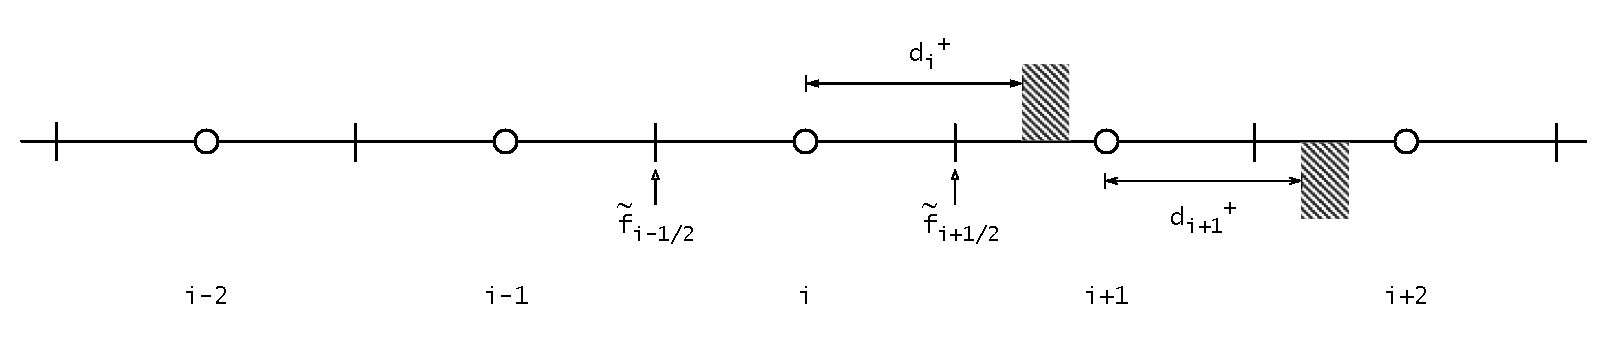
\includegraphics[width=15cm,clip]{stencil_case3.eps}
\end{center}
\caption{$\tilde{f}_{i+1/2}$評価時の$u_{\,i+1/2}<0$の場合の修正の判定.}
\label{fig:stencil case 3}
\end{figure}

%
\subsubsection{粘性項の計算}
粘性項を二次精度の中心差分で近似する場合は,\textbf{図\ref{fig:stencil case 1}}などでセル$(i-1,\,i+1)$について,壁面の影響を考慮して参照値の修正をすればよい.
あとは,参照値を用いて通常どおりのスキームにより計算をする\footnote{実装としては,壁面の影響を修正する処理を二重にするのを避けるため,対流項スキームとは分けず同一関数内で処理する.}.

%
\subsubsection{速度ベクトル発散の計算}
Poisson方程式のソース項や収束判定に用いる速度ベクトルの発散の計算について説明する.
\textbf{図\ref{fig:div operator}}に示すセルaは通常のステンシルで計算できる.一方,セルbとセルcは壁面の影響があるので,参照値を修正する.
修正の方法は前述した方法を適用する.

\begin{figure}[htbp]
\begin{center}
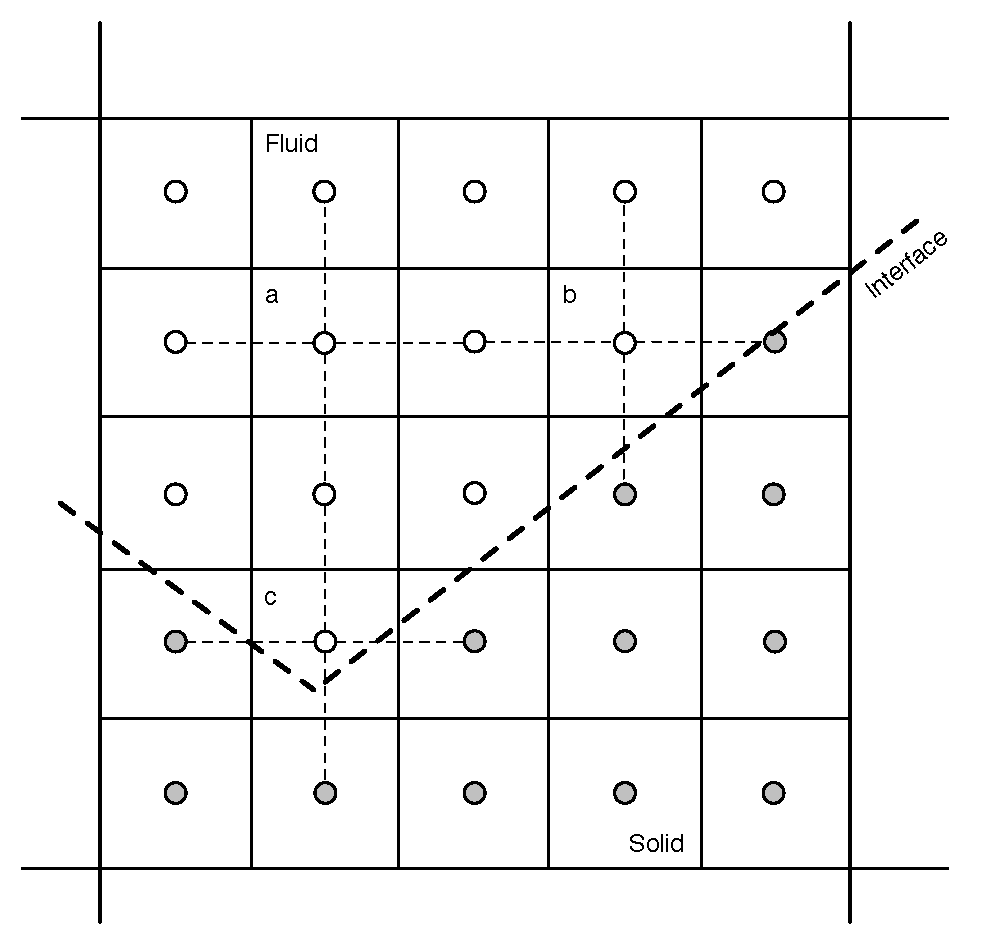
\includegraphics[width=10cm,clip]{div_operator.eps}
\end{center}
\caption{$\partial u_i / \partial x_i$の計算と圧力計算.○はセルセンター位置が流体で計算するセル,●は計算しないセル.aは通常のステンシル,セルb,cにはそれぞれ2方向,3方向の修正が必要.}
\label{fig:div operator}
\end{figure}

%
\subsection{圧力計算}
圧力計算の方法として,\hyperlink{tgt:Poisson Binary}{Binary近似}の方法と法線情報を用いて形状近似度を改善する方法が適用可能.

%
\subsubsection{バイナリ近似の前処理}
距離情報を用いた計算で圧力をバイナリで扱う場合,前処理時に距離情報を用いて\hyperlink{tgt:EBCS poisson BC}{ノイマン条件}をセットしておく.
各セル定義点で計算された6方向の距離情報をみて,それらが1.0\footnote{格子幅$\Delta x$で正規化.}でなければ壁面が存在することになる.

%
\subsubsection{法線を利用した参照点への内挿}
法線情報を用いて精度を改善する方法について述べる.


%
\subsection{物体との交点を含むセル間の速度ベクトルの内挿}
セルセンター速度からセルフェイス速度への内挿処理が必要になるが,物体との交点を含むセル間では注意する必要がある.
\textbf{図\ref{fig:interpolation cc2cf}}には,セル{i}の両側のセルフェイス位置の速度$\varphi_{\,i+1/2}, \varphi_{\,i-1/2}$に内挿する処理を示している.
左右のセルフェイスへは,それぞれ次式で内挿する.

\begin{equation}
\displaystyle{ \varphi_{\,i\pm1/2} \,=\, \frac{1}{d_i^{\pm}} \left[ \frac{1}{2} \varphi_{\,w} + \left( d_i^{\pm} - \frac{1}{2} \right) \varphi_{\,i} \right] }\\
\label{eq:interpolation cc2cf}
\end{equation}


\begin{figure}[htbp]
\begin{center}
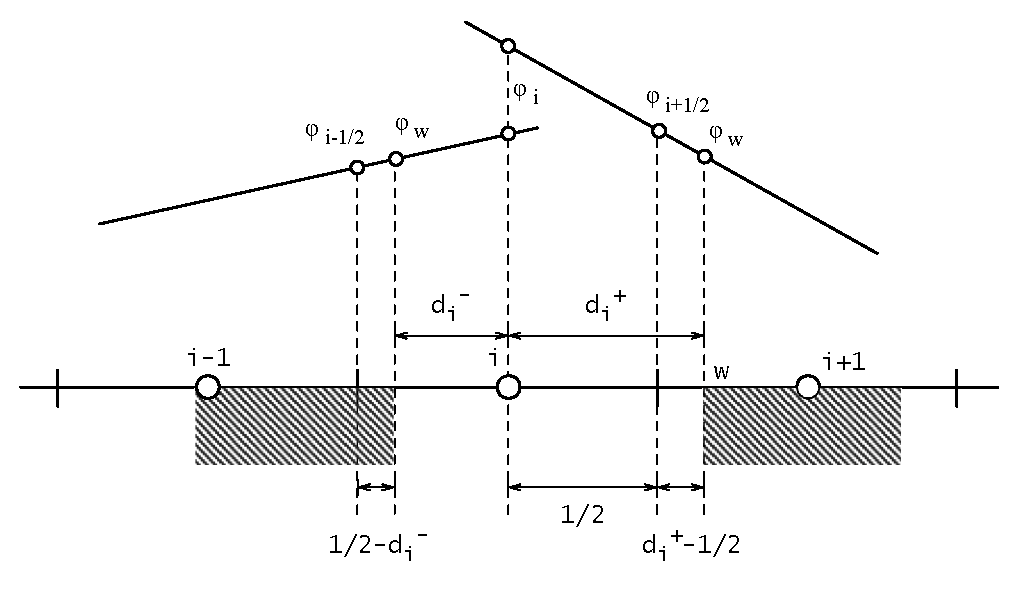
\includegraphics[width=11cm,clip]{intp_cut.eps}
\end{center}
\caption{セルセンターの速度ベクトルからセルフェイスの速度ベクトルへの内挿.}
\label{fig:interpolation cc2cf}
\end{figure}

セル間に薄い物体がある場合には,共有する同一のセル界面でも異なる参照値をもつことになる.
この場合には,セルフェイスの値を保持して,それを積分するやり方ではなく,セルセンターの値に直接積分して集約するようにする.
また,ここで述べる方法は\hyperlink{tgt:modify by cut}{前述した方法}とは異なるので,暫定的な実装.

\pagebreak

%%%
\section{体積力を用いた境界条件}
複雑形状周りの流れを解析する場合,Cartesian Methodは格子作成の労力を低減できる点で魅力的な方法である.
格子生成の手間は減少するが,それと引き換えにソルバー側で任意の形状の境界条件を取り扱う工夫が必要になる.
また,形状近似のレベルに応じて必要な形状パラメータを得る前処理プログラムの開発が必要となる.
Cartesian Methodでは格子密度が重要なパラメータとなるが,計算機資源や計算時間の制限から十分な格子が得られない場合がある.
現象の中に空間スケールの異なる流れがあり相互に影響するような問題,例えば,多孔質層を通過する大空間の流れを解析する場合,興味の対象は大空間内の流動挙動であり,多孔質層内はマクロに見て適切な流れ場になっていればよい.
この場合,多孔質部分はダルシー則などによりモデル化される.
メッシュ解像度以下の微細な構造が流動特性に与える影響は,ダルシー則などのように理論的,あるいは実験式などで与えられる場合も多い.
自動車のエンジンルーム内の流れを解析する場合にも,エンジンルーム内に配置される熱交換器は同様の特徴をもち,その特性は通過風速と圧力損失量の関係として実験式で与えられる.
本節ではCartesian Methodで有用な\hypertarget{tgt:body_force_bc}{体積力を用いた種々の境界条件}の導入について述べる.

%
\subsection{外力項による境界条件の導入}
\label{sec:external force method}

\textbf{式(\ref{eq:NS_ext_force ND})}に示すNavier-Stokes方程式中の外力項$F_{i}$を通して,体積力の形で様々な効果を導入する.各論の前に,まずFractional Step法に従って,大まかな手順を示す.

\begin{equation}
{\frac{\partial u_{i}}{\partial t}}^{n+1} + \frac{\partial}{\partial x_{j}} \left({ u_{i} u_{j} }\right)
\, =\,
- \frac{\partial p}{\partial x_{i}} + \frac{1}{Re} \frac{\partial}{\partial x_{j}} 
\left({ \frac{\partial u_{i}}{\partial x_{j}} + \frac{\partial u_{j}}{\partial x_{i}} }\right) + F_{i}
\label{eq:NS_ext_force ND}
\end{equation}


体積力として与える境界条件の位置は,ボクセルモデルのセル毎に付与されるIDにより指定される.
このIDにより,境界条件の種類と計算空間内の場所が特定できる.
この境界条件は,コンポーネントとして扱う\footnote{コンポーネントは,計算空間内に配置される境界条件や媒質を扱うための仕組みである.}.
体積境界条件コンポーネントの占有率$\beta$をセル中心で次のように定義する.

\begin{equation}
\left \{
\begin{array}{ll}
\beta \,=\, 0.0 & (Fluid)\\
0.0\le \beta \le 1.0 & (Component) \end{array}
\right. 
\label{eq:component fraction}
\end{equation}

$\beta$を用いると,\textbf{式(\ref{eq:NS_ext_force ND})}は次のように書ける.外力項を時間に関して陽的に扱う場合,非定常性が強い場合には不安定になることが懸念されるため,外力項を陰的に扱いPoissonの反復過程に組み込む.

\begin{equation}
{\frac{\partial u_{i}}{\partial t}}^{n+1} + \frac{\partial}{\partial x_{j}}{\left({ u_{i} u_{j} }\right)}^{n}
\, =\,
- {\frac{\partial p}{\partial x_{i}}}^{n+1} + \frac{(1-\beta)}{Re} \frac{\partial}{\partial x_{j}} \left({ {\frac{\partial u_{i}}{\partial x_{j}}}^{n} + {\frac{\partial u_{j}}{\partial x_{i}}}^{n} }\right) + \beta {F_{i}}^{n+1}
\label{eq:NS_ext_force ND2}
\end{equation}

Euler 陽解法を用いると疑似ベクトルは,

\begin{equation}
{u_{i}}^{*}
\, =\, 
{u}_{i}^{n}\, -\,\mathrm{\Delta}{t} \left\{{ \frac{\mathrm{\partial}}{\mathrm{\partial}{x}_{j}}{\left({{u}_{i}{u}_{j}}\right)}^{\hspace{0.3em}{n}}\mathrm{{-}}\,\frac{(1-\beta)}{Re} \frac{\partial}{\partial x_{j}} \left({ {\frac{\partial u_{i}}{\partial x_{j}}}^{n} + {\frac{\partial u_{j}}{\partial x_{i}}}^{n} }\right) }\right\}
\label{eq:pseudo_vector forcing}
\end{equation}

射影ステップは,
\begin{equation}
{u_{i}}^{n+1} \,=\, {{u}_{i}}^{*} - \Delta{t} \left({ {\frac{\partial p}{\partial x_{i}}}^{n+1} - \beta {F_{i}}^{n+1} }\right)
\label{eq:projection forcing}
\end{equation}

圧力反復は連続の式から導かれ,次のようになる.

\begin{equation}
\frac{\partial}{\partial x_i} {\left( \frac{\partial p}{\partial x_i} \right)}^{n+1}
\,=\,
\frac{1}{\Delta t} \frac{ {\partial u_i}^*}{\partial x_i}
\,+\,
\frac{\partial}{\partial x} \left( \beta {F_i}^{n+1} \right)
\label{eq:iteration forcing}
\end{equation}

\vspace{3mm}


多孔質内における流動は,対流項の影響よりも粘性力の影響が大きく,ダルシー抵抗と圧力のバランスが重要になる.\textbf{式(\ref{eq:iteration forcing})}による外力の扱いはこの事実を直接的に反映しており,多孔質内流動などではより早い収束が期待できる.


%
\subsection{熱交換器(圧力損失部)}
熱交換器の特性を想定した圧力損失モデルを外力項の形式で表し,\textbf{\ref{sec:external force method}}に示した計算アルゴリズム中にコンシステントに組み込む.
熱交換器は\textbf{図\ref{Heat exchanger}}のようにチューブとフィンから構成され,熱交換器面に対して面直の法線方向に流れが限定される.熱交換器の流動特性として,平均通過風速と熱交換器部で発生する静圧損失のマクロな関係がJISで定められる測定により得られる.これは\textbf{図\ref{pressure drop}}に示すようにほぼ二次関数としてモデル化できる.
熱交換器モデルとしては,下記の特性をもつ数値モデルを考える.

\begin{figure}[htbp]
  \begin{minipage}{.47\textwidth}
  	\begin{center}
  	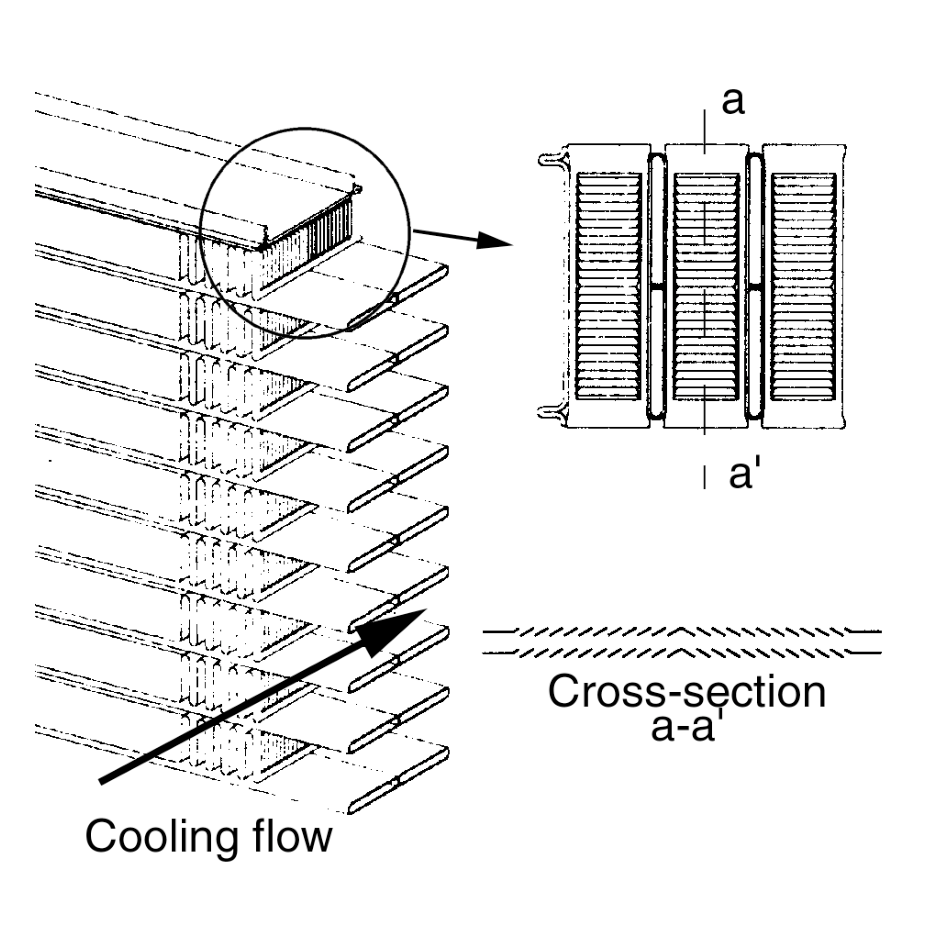
\includegraphics[width=8cm,clip]{HeatExchanger.eps}
  	\end{center}
  	\caption{自動車用熱交換器の構造}
	\label{Heat exchanger}
  \end{minipage} \hfill
  \begin{minipage}{.47\textwidth}
	\begin{center}
  	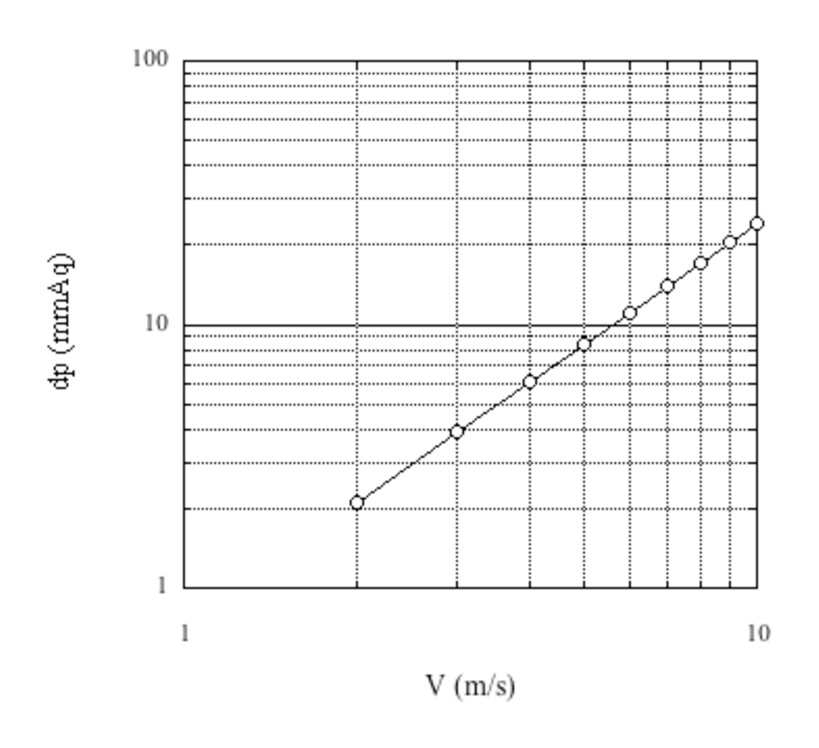
\includegraphics[width=7.5cm,clip]{Pressureloss.eps}
  	\end{center}
  	\caption{熱交換器の通過風量(風速)と圧力損失量の測定値}
  	\label{pressure drop}
  \end{minipage}
\end{figure}

\begin{itemize}
\item 流れの方向は法線${n_{i}}^{\prime}$方向(\textbf{図\ref{Heat exchanger}}中の矢印の方向)に限定される.
マクロな視点から${n_{i}}^{\prime}$と垂直方向には,チューブにより流れが発生しない.
\item ${n_{i}}^{\prime}$ 方向に$\Delta p^{\prime} = f({u_{i}}^{\prime})$の圧力損失が発生する.
\item 関数形として二次多項式の形式と離散データ形式を考慮する.
\item 熱交換器部では,傾斜して配置された場合の入口損失なども実験式に含まれることとする.
\end{itemize}

以下の基礎式を考える.

\begin{equation}
{\frac{\partial{{u}_{i}}^{\prime}}{\partial{{x}_{i}}^{\prime}}}^{n+1} \, =\, {0}
\label{eq:continuity_pl}
\end{equation}

\begin{equation}
{\frac{\partial{u_{i}}^{\prime}}{\partial{t}^{\prime}}}^{n+1} + \frac{\partial}{\partial{x_{j}}^{\prime}} \left({ {u_{i}}^{\prime} {u_{j}}^{\prime} }\right)
\, =\,
- \frac{\partial{p}^{\prime}}{\partial{x_{i}}^{\prime}} + \frac{\partial {\tau_{ij}}^{\prime}}{\partial{x_{j}}^{\prime}}
\label{eq:NS1_pl}
\end{equation}

\begin{equation}
{\tau_{ij}}^{\prime}
\,=\,
\nu \left({ \frac{\partial{u_{i}}^{\prime}}{\partial{x_{j}}^{\prime}} + \frac{\partial{u_{j}}^{\prime}}{\partial{x_{i}}^{\prime}} }\right)
\label{eq:tensor_pl}
\end{equation}

熱交換器部分では粘性項の影響を無視し,熱交換器による圧力損失の影響を${F_{R}}_{i}^{\prime}$とすると,

\begin{equation}
{\frac{\partial{u_{i}}^{\prime}}{\partial{t}^{\prime}}}^{n+1} + \frac{\partial}{\partial{x_{j}}^{\prime}} \left({ {u_{i}}^{\prime} {u_{j}}^{\prime} }\right)
\, =\,
- {\frac{\partial{p}^{\prime}}{\partial{x_{i}}^{\prime}}}^{R} + {F_{R}}_{i}^{\prime}
\label{eq:NS2_pl}
\end{equation}

ここで,圧力勾配項は熱交換器による静圧変化分を表す.
熱交換器の占有率として\textbf{式(\ref{eq:component fraction})}の$\beta$を用い,\textbf{式(\ref{eq:NS1_pl})}と\textbf{式(\ref{eq:NS2_pl})}をまとめると,

\begin{equation}
{\frac{\partial{u_{i}}^{\prime}}{\partial{t}^{\prime}}}^{n+1} + \frac{\partial}{\partial{x_{j}}^{\prime}} \left({ {u_{i}}^{\prime} {u_{j}}^{\prime} }\right)
\, =\,
- {\left\{{ \beta {\frac{\partial{p}^{\prime}}{\partial{x_{i}}^{\prime}}}^{R} + (1-\beta) \frac{\partial{p}^{\prime}}{\partial{x_{i}}^{\prime}} }\right\}}^{n+1} + (1-\beta) \frac{\partial{\tau_{ij}}^{\prime}}{\partial{x_{j}}^{\prime}}
\label{eq:NS3_pl}
\end{equation}

$\beta=0.0$のとき,つまり流体部分では,\textbf{式(\ref{eq:NS3_pl})}は\textbf{式(\ref{eq:NS1_pl})}と等価である.

ここで,熱交換器の圧力損失について考える.
コア厚さ$\Delta r^{\prime}$の熱交換器で${\Delta p^{\prime}}^{R}\, =\, f({{u_{i}}^{\prime}}^{R})$の圧力損失が得られる.
圧力損失は速度に比例して大きくなり,通常の圧力勾配と同じ符号となる.
つまり,正の向きの速度ベクトルに対して逆圧力勾配となる.

\begin{equation}
{F_{R}}_{i}^{\prime} \, =\,
-{sgn} \left({ {u_{i}}^{\prime} }\right) {\frac{\Delta{p}^{\prime}}{\Delta{r}^{\prime}}}^{R} {n_{i}}^{\prime}
\label{eq:Ploss_pl}
\end{equation}


\textbf{式(\ref{eq:Ploss_pl})}の無次元化にあたり,$sgn{({u_{i}}^{\prime})}, \, {n_{i}}^{\prime}$は単に方向を表すものであるので,無次元化には影響しない点に注意する.
熱交換器部の圧力勾配は,流れ場の圧力勾配に対して線形な関係を仮定すると,次のようにモデル化できる.

\begin{equation}
\frac{{\partial{p}^{\prime}}^{R}}{\partial{x_{i}}^{\prime}}
\, =\,
\frac{\partial{p}^{\prime}}{\partial{x_{i}}^{\prime}} + {F_{R}}_{i}^{\prime}
\label{eq:Ploss2_pl}
\end{equation}

\begin{equation}
{\frac{\partial{u_{i}}^{\prime}}{\partial{t}^{\prime}}}^{n+1} + \frac{\partial}{\partial{x_{j}}^{\prime}} \left({ {u_{i}}^{\prime} {u_{j}}^{\prime} }\right)
\, =\,
- {\frac{\partial{p}^{\prime}}{\partial{x_{i}}^{\prime}}}^{n+1} + (1-\beta) \frac{\partial{\tau_{ij}}^{\prime}}{\partial{x_{j}}^{\prime}} + \beta {{F_{R}}_{i}^{\prime}}^{n+1}
\label{eq:NS4_pl}
\end{equation}

\textbf{式(\ref{eq:NS4_pl})}を無次元化すると,\textbf{式(\ref{eq:NS_ext_force ND})}の形式になる.

%
\subsubsection{熱交換器の境界条件}
熱交換器に特有の境界条件として,\textbf{式(\ref{eq:projection_pl})}に従い,速度ベクトルを熱交換器の流出方向(面法線ベクトル${n_{i}}^{\prime}$)へ射影する.

\begin{equation}
{u_{i}}^{*}
\, =\,
(1-\beta) {u_{i}}^{*} \,+\, \beta \left|{ {u_{i}}^{*} }\right| n_{i}
\label{eq:projection_pl}
\end{equation}

もし,単に\textbf{式(\ref{eq:projection_ng_pl})}により方向を強制すると,ベクトルの成す角度が大きくなった場合,内積の値が小さくなり,速度ベクトルの大きさが小さくなる.そうすると,保存則を満たすように逆に圧力勾配が大きくなり熱交換器部分で加速するようになる.したがって,動圧が変化しないように\textbf{式(\ref{eq:projection_pl})}を採用する.

\begin{equation}
{u_{i}}^{*}
\, =\,
(1-\beta) {u_{i}}^{*} + \beta \left({ {u_{i}}^{*} n_{i} }\right) n_{i}
\label{eq:projection_ng_pl}
\end{equation}

\noindent $\beta$と$F_{i}$の各値は,速度ベクトル成分のセルセンタの点で定義されることに注意する.

熱交換器内部では,\textbf{式(\ref{eq:iteration forcing})}の右辺第3項もゼロになる.したがって,Laplace 方程式を解いていることになり,単に前後の圧力差から平滑化を行うことになる.これは,熱交換器の前後で圧力勾配の跳びが発生し,内部は流速一定の流れ場になっているとする仮定とコンシステントである.\textbf{式(\ref{eq:iteration forcing})}を解いて得られた圧力場は,熱交換器部で通過風速に応じた圧力勾配となっている.

本手法は流体の圧力場の一部分の勾配を指定しながら Poisson 方程式を解いている.これは,圧力 Poisson 方程式中において勾配の境界条件を満たすように解いていることと同じで,Liuら\cite{Liu:00:JCP}の Laplace/Poisson 方程式への境界条件の導入方法と基本的に同じアイデアである.また,圧力と速度の同時緩和を行いながら圧力損失項をアップデートするため,n+1 ステップでより良い近似になっている.


%
\subsubsection{圧力損失パラメータ}
圧力損失パラメータは,熱交換器の性能試験結果により得られる.$\Delta p-V$ の性能線図を$[mmAq - m/s]$ 単位とした場合のパラメータの取得について示す.\textbf{図\ref{pressure drop}}のように横軸に熱交換器の平均通過流速 $V^{\prime} [m/s]$, 縦軸に圧力損失ヘッド $h^{\prime} [mmAq]$ とする.多くの場合,流速の二次曲線で近似できる.プライム[$\,^{\prime}$] は有次元量を示すものとして,

\begin{equation}
{h}^{\prime} 
\,=\,
\left\{{ \begin{array}{ll}
c_{1} {u^{\prime}}^{2} \,+\, c_{2} u^{\prime} \,+\, c_{3} & \left({ u^{\prime} \geq {u_{th}}^{\prime} }\right)\\
c_{4} {u^{\prime}}^{2} & \left({ u^{\prime} < {u_{th}}^{\prime} }\right)
\end{array}}\right. \quad [mm]
\label{eq:coef1_pl}
\end{equation}

\noindent 係数$c_{4}$の式は速度が小さいときに圧力損失量をゼロに漸近させるためのもので,閾値${u_{th}}^{\prime}$で切り替える.\\

圧力損失と$\Delta r^{\prime} \,[mm]$の厚さの熱交換器部での圧力勾配は次のようになる.

\begin{equation}
{\Delta p}^{\prime} \,=\, {\rho_{w}}^{\prime} g h^{\prime} \times 10^{-3} \quad [Pa]
\label{eq:coef2_pl}
\end{equation}

\begin{equation}
\frac{{\Delta p}^{\prime}}{{\Delta r}^{\prime}} \,=\,\frac{{\rho_{w}}^{\prime} g h^{\prime}}{{\Delta r}^{\prime}} \quad [Pa/m]
\label{eq:coef3_pl}
\end{equation}

\noindent ${\rho_{w}}^{\prime}$は水の密度$[kg/m^3]$, $g$ は重力加速度 $[m/s^2]$ である.これらを次式で無次元化する.

\begin{equation}
\left.{ 
\begin{array}{l}
\vspace{2mm}
\Delta p \,=\, \displaystyle{ \frac{\Delta p^{\prime}}{{\rho_{0}}^{\prime} {u_{0}}^{2}} }\\
\vspace{2mm}
\displaystyle { \Delta r \,=\, \frac{\Delta r^{\prime}}{L^{\prime}} }\\
\vspace{2mm}
\displaystyle { u \,=\, \frac{u^{\prime}}{{u_{0}}^{\prime}} }
\end{array} \quad }\right\}
\label{eq:coef4_pl}
\end{equation}

\noindent 無次元の熱交換器部の圧力勾配は,基準密度を${\rho_{0}}^{\prime}$として,

\begin{equation}
\frac{\mathrm{\Delta}{p}}{\mathrm{\Delta}{r}}
\,=\,
\frac{ {\rho_{w}}^{\prime} {g} {h}^{\prime}} {\Delta{r}^{\prime}} \frac{L^{\prime}} {{\rho_{0}}^{\prime} {{u_{0}}^{\prime}}^{2}}
\label{eq:coef5_pl}
\end{equation}

\noindent これより,

\begin{equation}
{h}^{\prime} \equiv \left({ \frac{ \Delta p}{ \Delta r} }\right) \frac{{\rho_{0}}^{\prime}}{{\rho_{w}}^{\prime}}\frac{\Delta {r}^{\prime} {{u_{0}}^{\prime}}^{2}} {L^{\prime} g}
\,=\,
c_{1} {\left({ u\, {u_{0}}^{\prime} }\right) }^{2} \,+\, c_{2} \left({ u\, {u_{0}}^{\prime} }\right)  \,+\, c_{3}
\label{eq:coef6_pl}
\end{equation}

\begin{equation}
\frac{\Delta p}{\Delta r} 
\,=\,
\frac{{\rho_{w}}^{\prime} L^{\prime} g} {{\rho_{0}}^{\prime} \Delta r^{\prime} {{u_{0}}^{\prime}}^{2}} 
\left\{{ 
c_{1} {\left({ u\, {u_{0}}^{\prime} }\right) }^{2} \,+\, c_{2} \left({ u\, {u_{0}}^{\prime} }\right)  \,+\, c_{3}
}\right\}
\,=\,
\frac{{\rho_{w}}^{\prime} L^{\prime} g} {{\rho_{0}}^{\prime} \Delta r^{\prime}} \left({
c_{1} u^{2} \,+\, \frac{c_{2}}{{u_{0}}^{\prime}} u \,+\, \frac{c_{3}}{{{u_{0}}^{\prime}}^{2}}
}\right)
\label{eq:coef7_pl}
\end{equation}

\noindent 係数を\textbf{式(\ref{eq:coef8_pl})}でまとめると,

\begin{equation}
\left.{
\begin{array}{l}
\vspace{2mm}
\displaystyle{ \xi_{1} \,=\, \frac{ {\rho_{w}}^{\prime} L^{\prime} g} { {\rho_{0}}^{\prime} \Delta r^{\prime}} c_{1} }\\
\vspace{2mm}
\displaystyle{ \xi_{2} \,=\, \frac{ {\rho_{w}}^{\prime} L^{\prime} g} { {\rho_{0}}^{\prime} \Delta r^{\prime}} \frac{c_{2}}{{u_{0}}^{\prime}} }\\
\vspace{2mm}
\displaystyle{ \xi_{3} \,=\, \frac{ {\rho_{w}}^{\prime} L^{\prime} g} { {\rho_{0}}^{\prime} \Delta r^{\prime}} \frac{c_{3}}{{{u_{0}}^{\prime}}^{2}} }\\
\vspace{2mm}
\displaystyle{ \xi_{4} \,=\, \frac{ {\rho_{w}}^{\prime} L^{\prime} g} { {\rho_{0}}^{\prime} \Delta r^{\prime}} c_{4} }
\end{array} \quad }\right\}
\label{eq:coef8_pl}
\end{equation}

\noindent 無次元の圧力勾配は\textbf{式(\ref{eq:coef9_pl})}で表せる.

\begin{equation}
\frac{\mathrm{\Delta}{p}}{\mathrm{\Delta}{r}} \mathrm{{=}} \left\{{\begin{array}{ll}
{{\mathit{\xi}}_{1}{u}^{2} \,+\, {\mathit{\xi}}_{2}{u} \,+\, {\mathit{\xi}}_{3}} & {\left({{u}\hspace{0.33em}\mathrm{\geq}\hspace{0.33em}{u}_{th}}\right)}\\
{{\mathit{\xi}}_{4}{u}^{2}} & {\left({{u}\hspace{0.33em}{\mathrm{<}}\hspace{0.33em}{u}_{th}}\right)}\end{array}}\right.
\label{eq:coef9_pl}
\end{equation}

\noindent 無次元の圧力勾配から有次元の圧力損失量へは\textbf{式(\ref{eq:coef5_pl})}を用いて算出する.\vspace{5mm}


圧力損失ヘッドの測定単位が $p^{\prime}\: [mmHg]$ の場合には,水の密度を水銀密度$\rho_{mercury}^{\prime}$ に変更する\footnote{mmAqの場合には,$\theta =300 [K],\,p=101.325 [kPa]$で,$\rho_{water}^{\prime}=996.62 [kg/m^3]$,mmHgの場合には,$\theta =300 [K]$で,$\rho_{mercury}^{\prime}=13538 [kg/m^3]$をハードコード.}.
圧力損失が$\Delta p^{\prime}\: [Pa]$で与えられる場合には,

\begin{equation}
\Delta p^{\prime}
\,=\,
\left\{{ \begin{array}{ll}
c_{1} {u^{\prime}}^{2} \,+\, c_{2} u^{\prime} \,+\, c_{3} & \left({ u^{\prime} \geq {u_{th}}^{\prime} }\right)\\
c_{4} {u^{\prime}}^{2} & \left({ u^{\prime} < {u_{th}}^{\prime} }\right)
\end{array} \quad }\right. [Pa]
\label{eq:coef10_pl}
\end{equation}

\begin{equation}
\frac{\mathrm{\Delta}{p}}{\mathrm{\Delta}{r}}
\,=\,
\frac{\Delta p^{\prime}}{\Delta r^{\prime}} \frac{L^{\prime}} {{\rho_{0}}^{\prime} {{u_{0}}^{\prime}}^{2}}
\label{eq:coef11_pl}
\end{equation}

\begin{equation}
\Delta p^{\prime} \equiv \left({ \frac{\Delta p}{\Delta r} }\right) \frac{\Delta r^{\prime}}{L^{\prime}} \rho_{0}^{\prime}{{u_{0}}^{\prime}}^{2}
\,=\,
c_{1} {\left({ u\, {u_{0}}^{\prime} }\right) }^{2} \,+\, c_{2} \left({ u\, {u_{0}}^{\prime} }\right)  \,+\, c_{3}
\label{eq:coef12_pl}
\end{equation}

\begin{equation}
\frac{\Delta p}{\Delta r}
\,=\,
\frac{L^{\prime}}{{\rho_{0}}^{\prime} \Delta r^{\prime} {{u_{0}}^{\prime}}^{2}} \left\{{ 
c_{1} {\left({ u\, {u_{0}}^{\prime} }\right) }^{2} \,+\, c_{2} \left({ u\, {u_{0}}^{\prime} }\right)  \,+\, c_{3}
}\right\}
\,=\,
\frac{L^{\prime}}{{\rho_{0}}^{\prime} \Delta r^{\prime}} \left({ 
c_{1} u^{2} \,+\, \frac{c_{2}}{{u_{0}}^{\prime}} u \,+\, \frac{c_{3}}{{{u_{0}}^{\prime}}^{2}}
}\right)
\label{eq:coef13_pl}
\end{equation}

\begin{equation}
\left.{
\begin{array}{l}
\vspace{2mm}
\displaystyle{ \xi_{1} \,=\, \frac{ L^{\prime}} { {\rho_{0}}^{\prime} \Delta r^{\prime}} c_{1} }\\
\vspace{2mm}
\displaystyle{ \xi_{2} \,=\, \frac{ L^{\prime}} { {\rho_{0}}^{\prime} \Delta r^{\prime}} \frac{c_{2}}{{u_{0}}^{\prime}} }\\
\vspace{2mm}
\displaystyle{ \xi_{3} \,=\, \frac{ L^{\prime}} { {\rho_{0}}^{\prime} \Delta r^{\prime}} \frac{c_{3}}{{{u_{0}}^{\prime}}^{2}} }\\
\vspace{2mm}
\displaystyle{ \xi_{4} \,=\, \frac{ L^{\prime}} { {\rho_{0}}^{\prime} \Delta r^{\prime}} c_{4} }
\end{array} \quad }\right\}
\label{eq:coef14_pl}
\end{equation}

%%
\subsubsection{実装の方針}
体積力コンポーネントには,下記のような特徴がある.
\begin{description}
\item[-] 一般に,コンポーネントは計算空間中に局在し,そのセル数も少ない.したがって,そのコンポーネントの計算に必要な体積率などを全空間にわたって保持する配列を用いるのはメモリコストがかかる.
\item[-] 局在性のため,並列処理時には負荷バランスが崩れることは避けられない.
\item[-] 必要な計算のために,体積率,重複計算を避けるためのワーク配列が必要.その配列の大きさは Bbox のサイズで与えられるが,前述のように全領域の中の一部分である.また,コンポーネントは一つでも全領域の配列が必要となる.
\end{description}

以上の点から,次の実装が考えられる.
\begin{description}
\item[-] ワーク配列を必要とするコンポーネントがある場合には,そのの配列 (dc\_wvex, dc\_cfr) を全空間にわたって確保する.各コンポーネントの Bbox の大きさはサーチ用に利用する.メモリの無駄が生じるが,並列処理は標準的な方法が利用可能.コンポーネント(熱交換器を含む一般的な要素)の占有率$\beta$は,バイナリボクセルの場合,BinaryVoxel::setCmpFractionBV() により, bcx[] の情報から生成し,cfr[] に保持する.
\item[-] 別の方法としては,各コンポーネントの Bbox の大きさの配列をアロケートし,体積率とワークに用いて計算する.これにより,メモリ効率と計算負荷を小さく抑えられる.また,一方で並列処理時のインデクスの計算などが煩雑になるが,V-Sphereのコンポーネント機能を用いて実装する\footnote{テスト実装を試みるが,きわめて複雑で断念...}.
\end{description}
ここでは,前者の方法で実装した.

BVHを使って絞り込みを行っているが,Hybrid並列ではOpenMPのループ分割でロードインバランスが生じる可能性が高いので,一次元配列をコア数で分割する方がよい.


%%
\subsubsection{解法の手順}

\begin{enumerate}
\item 圧力損失部の疑似速度ベクトルの修正\\
疑似速度ベクトルの計算式(\ref{eq:pseudo_vector forcing})を式(\ref{eq:pseudo2_pl})のように表し,流束の計算を通常の計算処理 (i) と圧力損失部分による修正 (ii) の2ステップに分解して計算する.
(ii) の計算は,コンポーネントリストクラスと bcd[] の情報を用いて対象部分のみ計算する.
実装では有限体積的に流束を評価しているので,修正も流束に対して行う.

\begin{equation}
\begin{array}{l}
\displaystyle { 
{u_{i}}^{*} 
\,=\, 
{u_{i}}^{n} - \Delta{t} \left\{{ \frac{\partial}{\partial{x}_{j}} {\left({ u_{i} u_{j} }\right) }^{n} - \frac{(1-\beta)}{Re}\frac{\partial}{\partial x_{j}} \left({ {\frac{\partial u_{i}}{\partial x_{j}}}^{n} + {\frac{\partial u_{j}}{\partial x_{i}}}^{n} }\right) }\right\} }\\
\displaystyle {\hspace{1.5em} = \, {u_{i}}^{n} - \Delta{t} \left[{ 
\underbrace{
\frac{\partial}{\partial{x}_{j}} {\left({ u_{i} u_{j} }\right) }^{n} 
- \frac{1}{Re} \frac{\partial}{\partial x_{j}} \left({ {\frac{\partial u_{i}}{\partial x_{j}}}^{n} + {\frac{\partial u_{j}}{\partial x_{i}}}^{n} }\right)
}\limits_{(i)}
\underbrace{ 
+ \frac{\beta}{Re} \frac{\partial}{\partial x_{j}} \left({ {\frac{\partial u_{i}}{\partial x_{j}}}^{n} + {\frac{\partial u_{j}}{\partial x_{i}}}^{n} }\right) }\limits_{(ii)} }\right] 
}
\end{array}
\label{eq:pseudo2_pl}
\end{equation}

\textbf{式(\ref{eq:projection_pl})}により,圧力損失部の疑似速度ベクトルを流出方向に修正する(\verb|SetBC3D::mod_Pvec_Forcing()|).
オプションとして,方向修正をしない場合も考慮する.

\vspace{2mm}

\item Poissonの圧力反復式とソース項の追加\\
圧力損失部は外力項としてNavier-Stokes方程式に組み込まれ,その発散量がPoisson方程式のソース項として作用する.
つまり,圧力の反復式には圧力損失が寄与するソース項として,\textbf{式(\ref{eq:iteration forcing})}の右辺第2項が追加される.
反復の半離散式は,\textbf{式(\ref{eq:poisson_iteration})}を参照して以下のようになる.

\begin{equation}
\left.
\begin{array}{lll}
\vspace{2mm}
\tilde{p} & = & \displaystyle { \frac{1}{\sum \limits_l \left( \, \phi^{\,N}_{\,l} \, \right)} 
\left \{ \,
\sum \limits_l {\left( p \,\phi^{\,D} \,\phi^{\,N}\right)}_{\,l} 
\underbrace{ \,-\, \gamma^{\,0} \,+\, \gamma^{\,D1} \,+\, \gamma^{\,N1} } \limits_{反復中固定値}
\underbrace{ \,+\, \gamma^{\,D2} \,+\, \gamma^{\,N2} \,-\, \gamma^{\,F} } \limits_{反復毎に変化}
\, \right \} } \\

\vspace{2mm}
\Delta p & = & \tilde{p} \,-\, p^{\,k} \\

\vspace{5mm}
p^{\,k+1} & = & p^{\,k} \,+\, \omega\, \,\Delta p \\

\vspace{2mm}
\gamma^{\,F} & = & \displaystyle{ h \sum \limits_l {\left( \beta F^{n+1} \right)}_{\,l} \,n_{\,l} } \\
\end{array} \qquad \right \}
\label{eq:poisson itr w/forcing}
\end{equation}

ここで,$\gamma^{\,F}$が圧力損失部によるソース項を表し,\verb|SetBC3D::mod_Psrc_Forcing()|で計算している.
反復プロセスは圧力と速度の同時緩和を採用しているので,$\gamma^{\,F}$の項は反復毎に計算する.
これは外力成分の発散を表しているので,各成分はセルフェイス位置で評価する.このため,セルセンターで定義された$F_i$の算術平均をとり,セルフェイス位置に内挿する.つまり$i+1/2$の場合には,次式を用いる\footnote{赤坂 啓,小野 謙二:直交格子を用いた非圧縮流れ解析における圧力損失モデルの実装, Transaction of JSCES, 20070032(2007)}.

\begin{equation}
{\left( \beta F_1^{\,n+1} \right)}_{i+1/2} \, =\,
\frac{\beta_{i+1}+\beta_i}{2} \frac{F_{1,\,i+1}^{\,n+1} + F_{1,\,i}^{\,n+1}}{2}
\label{eq:F_R interpolation}
\end{equation}

圧力損失による外力は\textbf{式(\ref{eq:Ploss_pl})}で表される.無次元で表記すると,

\begin{equation}
{F_i}^{\,n+1} \, =\,
-{sgn} \left({ u_i^{\,n+1} }\right) {\frac{\Delta p}{\Delta r}}^{n+1} \, n_i
\label{eq:Ploss_pl_ND}
\end{equation}

ここで,$F_i$の各成分はセルセンターで定義されることに注意する.
無次元圧力勾配の評価には,\textbf{式(\ref{eq:coef9_pl})}を用いる.
\vspace{2mm}

\item 圧力損失部の速度ベクトルの射影\\
射影ステップは,式(\ref{eq:projection forcing})を式(\ref{eq:projection forcing decomp})の(i), (ii)の2ステップに分解し,(ii)の修正項をコンポーネントリストを参照しながら計算する.

\begin{equation}
{u_{i}}^{n+1} \,=\,  
\underbrace{ {u_{i}}^{*} - \Delta{t} \left({ \frac{\partial p}{\partial x_{i}^{n+1}} }\right) }\limits_{(i)}
\underbrace{ - \Delta{t} \beta {F_{i}}^{n+1} }\limits_{(ii)}
\label{eq:projection forcing decomp}
\end{equation}

セルセンターとセルフェイスの速度成分に対して,\textbf{式(\ref{eq:projection forcing})}を2段階に分けて各々\verb|SetBC3D::mod_Vcf_Forcing()|,\verb|SetBC3D::mod_Vcc_Forcing()|により処理する.
\begin{equation}
\begin{array}{l}
\displaystyle{ {u_{i}}^{n+1} \,=\, {{u}_{i}}^{*} - \Delta{t} {\frac{\partial p}{\partial x_i}}^{n+1} }\vspace{2mm}\\
\displaystyle{ {u_{i}}^{n+1} \,+=\, \Delta{t} \beta {F_{i}}^{n+1} }\vspace{2mm}\\
\end{array}
\label{eq:projection forcing2}
\end{equation}
\vspace{2mm}

\item 実装上のコメント\\
\begin{enumerate}
\item 外力項の計算\\
\textbf{式(\ref{eq:Ploss_pl_ND})}で評価する外力項と\textbf{式(\ref{eq:projection forcing2})}の外力項の値は同じである必要があるが,反復の過程で前反復値とほぼ同じになると考え,以下のようにコード化している.

\begin{indentation}{3zw}{0zw}
\begin{description}
\item[(1)] Poissonのソース項は前反復値 $F_i = f(u_i^k)$を使う.
\item[(2)] セルフェイスの速度の射影 $F_i = f(u_i^k)$
\item[(3)] セルセンターの速度の射影 $F_i = f(u_i^{k+1})$
\end{description}
\end{indentation}

この処理は,上記の全計算で$F_i = f(u_i^k)$を保証するためには,$F_i$の値を計算してベクトル配列に保持しておく必要があること,並列時に通信が発生することの2点を避けるためである.
\vspace{2mm}

\item 外力項のPoissonのソース項の扱い\\
セルフェイスの速度の射影ステップで,熱交換器部分の影響が\textbf{式(\ref{eq:projection forcing2})}のように入り,熱交換器を構成するセルの各面で外力項が作用する.
したがって,熱交換器の隣接セルについても,熱交換器に接するセルフェイスは影響を受ける.
このことは,ソース項を計算する場合,熱交換器の隣接セルについてもソース項を計算しておく必要があることを意味する.
\end{enumerate}

\vspace{2mm}

\item モニタ値の計算\\
モニタ量は,熱交換器部の通過風速と圧力損失量の無次元平均値を次式で計算する.$m$は熱交換器を構成するセル数である.

\begin{equation}
\begin{array}{lll}
\bar{u}_{hex}  &=& \displaystyle{  \frac{1}{m} \sum_m {sgn(n_i,u_i) \left| u \right| \beta} }\\
\displaystyle{\bar{\frac{\Delta p}{\Delta r}}_{hex}} &=& \displaystyle{ -\frac{1}{m} \sum_m {sgn(n_i,u_i) \, \frac{\Delta p}{\Delta r} \,\beta } }\\
\end{array}
\label{eq:hex monitor}
\end{equation}

圧力損失量は,熱交換器の厚さ方向の値を次式で推定し,有次元化して履歴に出力する.
\begin{equation}
\displaystyle{ \bar{\Delta p}_{hex} = \frac{\bar{\Delta p}}{\Delta r}\, {\Delta r} \, \rho {u_0^{\prime}}^2 L^{\prime} \quad [Pa]}\\
\label{eq:hex monitor2}
\end{equation}

\end{enumerate}

\pagebreak
%
\subsection{ファンモデル}
前述の圧力損失モデルと同様な方法でファンのP-Q特性を反映したマクロモデルを構築する.
ファンモデルは,圧力損失モデルと異なり,ファン回転の仕事により圧力増加(Pressure Gain)が生じ,また回転方向の流速が発生する.
最初に,軸流と斜流ファンに適用可能なファンモデル,その後,遠心ファンのモデルを説明する.

%
\subsubsection{ファン特性とモデル}
ファンの圧力増加と流量の関係,いわゆるP-Q特性はJISで定められた\textbf{図\ref{fig:chamber&p-q}}のチャンバー方式の測定方法により計測され,P-Q特性線図が得られる.
排気側にファンを設置し,流量を変化させた場合の圧力ゲインを測定する.圧力の測定はチャンバー内a点の静圧と大気圧の差を測定する.
ただし,チャンバー断面積は十分に大きく,チャンバー中央部a点での流速はほぼゼロに近いため,動圧はゼロと見なして良い.
したがって,a点付近で測定した静圧は全圧と等しいと考えて良い.

\begin{figure}[htdp]
\begin{minipage}{0.5\hsize}
\begin{center}
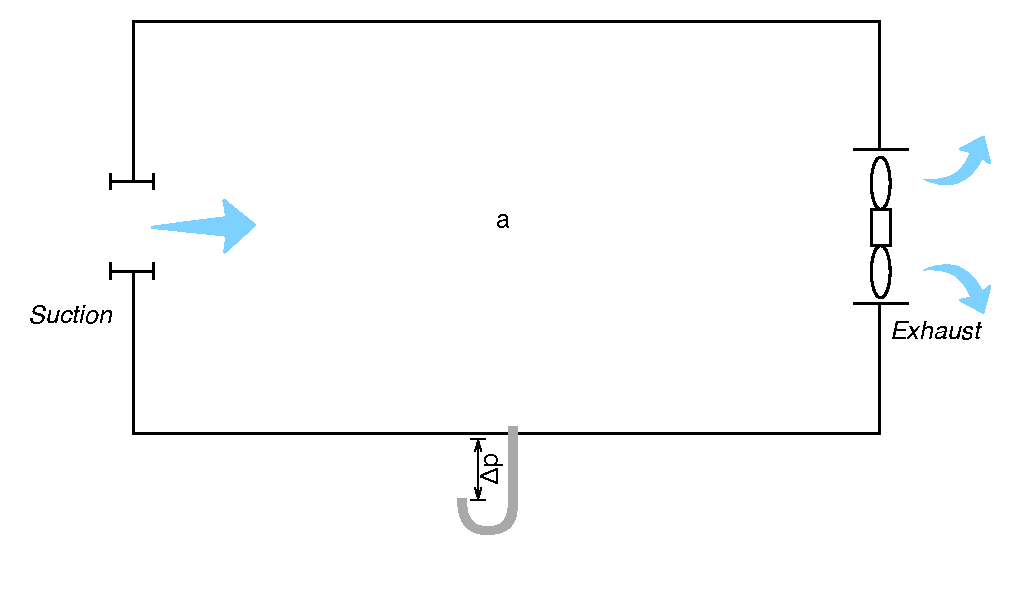
\includegraphics[width=8cm,clip]{chamber.eps}
\end{center}
\end{minipage}
\begin{minipage}{0.45\hsize}
\begin{center}
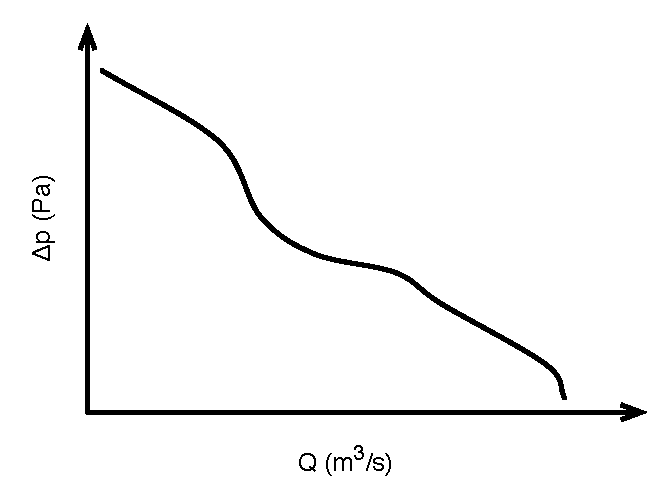
\includegraphics[width=6cm,clip]{fan-PQ.eps}
\end{center}
\end{minipage}
\caption{チャンバーによるファンの特性測定とP-Q線図.}
\label{fig:chamber&p-q}
\end{figure}

こうして得られたファンのP-Q特性を計算に用いる場合には,次の点に注意する必要がある.合わせて,CBCソルバーの実装方針も記す.
\begin{enumerate}
\item ファンの直近にある物体の影響\\
 ファン近傍に物体がある場合には,測定時の状況とはP-Q特性が異なるために適用には注意が必要となる.基本的にはファン前後の近距離には物体を配置しないことであるが,シュラウドのようにほぼ一体となっているものは,シュラウド込みで測定し,P-Q特性を取得するという利用方法も考えられる.
\vspace{2mm}

\item ラム圧の影響\\
 自動車の車載ファンのように走行風がある場合や,流路の狭い部分に設置されたファンの場合には,動圧の影響が無視できない.
この場合,動圧分の補正をしないとファンの動作点がずれていく.
計算モデルにおけるファン部分の上流側,下流側の位置をそれぞれ1,2で表し,静圧,動圧,全圧をそれぞれ$p_S,\,p_D,\,p_T\, (p_T = p_S + p_D)$とする.
圧力ゲインの計算方法として,測定データに基づく実装として,次の2通りが考えられる\footnote{ファン下流の速度が得られている場合には,$p_{T2}$を用いた方法も考えられるが,一般的な測定データとしては得られない.}.
\begin{enumerate}
\item ファン前後の静圧差で計算する.つまり,$\Delta p = p_{S2} - p_{S1}$.この実装では,動圧の影響を考慮できずに動サテンがずれる.
\item 上流側の全圧と下流側の静圧の差で計算する.つまり,$\Delta p = p_{S2} - p_{T1}$.この実装により,上流側の動圧の影響を取り込むことができる.
\end{enumerate}
CBCでは(b)の実装を行う.
\vspace{2mm}

\item 測定値の反映\\
計算では測定データを多項式近似によりモデル化する方法が採られる.一般的には,P-Q特性を一次式で近似することが多いが,一次式に乗らない点の影響が大きな場合がある.これは,多項式近似をしても根本的にはなくならない.そこで,CBCでは測定データ点をそのままテーブルとして保持し,データテーブルをピックアップしてP-Q特性を計算する.実装としては,\hyperlink{tgt:DH}{DataHolderクラス}を用いる.
\vspace{2mm}

\item 回転数や風量によるP-Q特性の補正\\
P-Q特性は定格回転数のみで有効である.回転数が異なる場合には補正したデータを用いる必要がある.
\[
\begin{array}{ll}
\vspace{2mm}
風量比  & \displaystyle{ \frac{Q_2}{Q_1} \,=\, \left( \frac{L_2}{L_1} \right)^3 \,\frac{N_2}{N_1} }\\
静圧比  & \displaystyle{ \frac{P_2}{P_1} \,=\, \left( \frac{L_2}{L_1} \right)^2 \,\left( \frac{N_2}{N_1} \right)^2 } \\
\end{array}
\]

ここで,$Q,\,L,\,N,\,P$はそれぞれ流量,ファンブレード径,回転数,静圧を表し,1,2は状態を表す.

\end{enumerate}


%
\subsubsection{旋回流}
ファンの軸流方向についてはP-Q特性でその流量(速度成分)が与えられるが,回転方向成分は何らかのモデルが必要となる.
よく使われる方法として,スリップ率を与える方法がある.スリップ率を一様に与える方法や半径方向の分布を与える方法などバリエーションは考えられるが,まず一様に与える方法を採用する.

ファンの通過風速については,流路面積を考慮する必要がある.つまり,ファンのボス部分は有効な通過面積ではないため,この部分の面積を除いた断面積を流路面積として扱う.これにより,同じ流量でも通過風速が異なり,動圧に反映され,P-Q特性のルックアップ値が異なるため,注意する.

熱解析の場合には,ファンボス部分の背後に設置されているモータが発熱体として指定されることもある.

さらに,ファン停止時には逆流も許すように流路部分がフリーとなるように考える.これは,外力項をゼロにすることで対応する.




%
\subsubsection{実装と解法の手順}


%
\subsubsection{遠心ファン}
遠心ファンでは,吸入部分と排気部分で流速の方向が異なり,上記の軸流タイプの実装ができない.
そこで,吸入部分と排気部分の速度ベクトルを規定し,圧力差をP-Q線図により与える実装とする.




\pagebreak
%
\subsection{多孔質体モデル}
\label{sec:porous model}
本節では,多孔質モデルの取り扱いについて説明する.

\subsubsection{Darcyモデル}

均質な空間に$A^{\prime}\,[m^2]\,\times\,L^{\prime}\,[m]$の直方体の検査体積を考える.両端の圧力差が$\Delta P^{\prime} \,[Pa]$で流量が$Q^{\prime}\,[m^3/s]$の場合,透過率(Permeability)を$k\,[m^2]$として,
\begin{equation}
Q^{\prime} \,=\, k \frac{A^{\prime}}{\mu} \frac{\Delta P^{\prime}}{L^{\prime}}
\label{Darcy's law 1}
\end{equation}

\begin{equation}
u^{\prime} \,=\, \frac{Q^{\prime}}{A^{\prime}} \,=\, \frac{k}{\mu} \frac{\Delta P^{\prime}}{L^{\prime}}
\label{Darcy's law 2}
\end{equation}

ここで,$\mu\,[Pa \cdot s]$は粘性係数,$u^{\prime}\,[m/s]$は見かけの通過流速(多孔質内の平均速度)である.$\Delta P^{\prime}/L^{\prime}$は圧力勾配なので,$u^{\prime}\,(\mu/k)$が力を表す.したがって,多孔質体部分の存在により流体に作用する外力は,

\begin{equation}
{F_{D}}_{\,i}^{\prime} \,=\, - {u_{i}}^{\prime} \frac{\mu}{k}
\label{NS_darcy_force}
\end{equation}

\textbf{式(\ref{NS_ext_force ND})}の形式に合わせて,$\rho^{\prime} {u_{0}^{\prime}}^{2}/L^{\prime}$で無次元化すると,

\begin{equation}
{F_{D}}_{\,i} \,=\, - \frac{1}{K}{u_{i}}
\label{NS_darcy_force_ND}
\end{equation}

ここで,$K$は無次元透過率を表す.
\begin{equation}
K \,=\, \frac{k}{\mu} \frac{\rho^{\prime} {u_{0}}^{\prime}}{L^{\prime}}
\label{permeability ND}
\end{equation}


\subsubsection{軸方向の異方性を考慮したDarcyモデル}

非等方性を考慮したDarcyモデルは\textbf{式(\ref{permeability aniso})}のように表せる.

\begin{equation}
{F_{D}}_{\,i}^{\prime} \,=\, - \frac{\mu}{k_{ji}}{u_{j}}^{\prime}
\label{permeability aniso}
\end{equation}

$k_{ji}$は異方性の係数を表すテンソルであるが,ここでは主軸方向の非等方性のみを考えるので,

\begin{equation}
k_{i} \,=\, 
\begin{pmatrix}
k_{1} & 0 & 0\\
0 & k_{2} & 0\\
0 & 0 & k_{3}
\end{pmatrix}
\label{permeability matrix}
\end{equation}

\textbf{式(\ref{permeability ND})}と同様に無次元化すると,

\begin{equation}
{F_{D}}_{\,i} \,=\, - \frac{1}{K_{i}} {u_{i}}
\label{NS_darcy aniso ND}
\end{equation}

Darcyモデルを用いる場合に必要なパラメータは\textbf{式(\ref{permeability matrix})}の主軸方向の成分となる.等方性の場合には,係数$k_{1},\,k_{2},\,k_{3}$に同じ値を与える.パラメータの記述については,\textbf{\ref{Darcy model param}}を参照.


%
\subsection{共通の前処理}
圧力損失,ファン,多孔質体の各境界条件は,基礎方程式の外力項としてモデル化している.
この外力項は各コンポーネントの体積占有率の情報を必要とする.
しばしば設計で用いられる不完全な入力形状データからコンポーネントの占有率を計算することは,内外判定に曖昧さが生じるため少々厄介である.
また,マクロモデルは実際の詳細な形状があったとしても,計算のために少々形状変更を行う必要もある.
そこで,モデルの特性と前処理のバランスを考慮して,以下の方針でモデル化し前処理を行う.

\begin{enumerate}
\item コンポーネントを矩形や円筒形に近似したボリュームとして扱い,体積占有率を自動計算する,
\vspace{2mm}

\item ボリュームを再現する幾何情報は数値データとして入力する.
幾何情報データをCADデータから読み取る作業は手間がかかるが,V-Xgenの機能として実装することも可能.
SVの場合にはボクセライズ時の内部データ構造に関係なく,直交等間隔となるので問題ないが,Octreeの場合にはダミーSTLを作成し,格子を細かくしておく必要がある.
\end{enumerate}

%
\subsubsection{入力幾何形状情報}
コンポーネントの幾何形状情報は\textbf{図\ref{fig:geometry_info}}に示すように,圧力損失部とファンのボリュームを構成する情報となる.
\begin{itemize}
\item 圧力損失部
{\small
\begin{equation}
\left.
\begin{array}{lll}
W  & 幅  &  [m] \\
H  & 高さ  & [m] \\
D  & 厚さ  & [m] \\
\overrightarrow{n} & 流出方向法線ベクトル成分 & [-] \\
\overrightarrow{d} & 幅方向ベクトル成分 & [-] \\
O_R & 前面の中心座標 & [m] \\
\end{array} \hspace{1cm} \right\}
\end{equation}
}

\item ファン
{\small
\begin{equation}
\left.
\begin{array}{lll}
R_F  & ブレード半径  &  [m] \\
R_B  & ボス半径  & [m] \\
D  & 厚さ  & [m] \\
\overrightarrow{n} & 流出方向法線ベクトル成分 & [-] \\
O_F & 前面の中心座標 & [m] \\
\end{array} \hspace{1cm} \right\}
\end{equation}
}

\end{itemize}


\begin{figure}[htbp]
\begin{center}
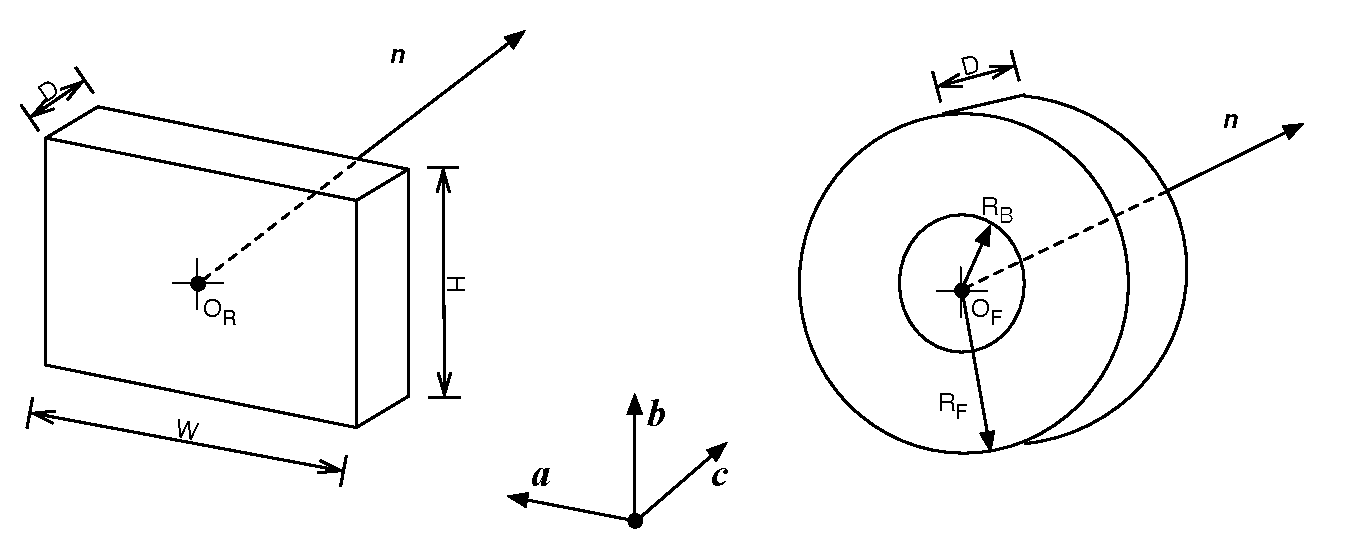
\includegraphics[width=12cm,clip]{compo_dim.eps}
\end{center}
\caption{圧力損失部とファン部の幾何情報.}
\label{fig:geometry_info}
\end{figure}

上記のジオメトリ情報から完全に閉じたボリューム形状を再構築できる.
また,\textbf{図\ref{fig:geometry_info}}の二つの形状は比較的簡単であり,プログラムで内外判定が可能である.

%
\subsubsection{占有率の計算}
コンポーネントの占有率の厳密な計算は難しいため,ある精度でサンプリングすることにより近似的に体積占有率を求める.
また,コンポーネントは空間内に任意の位置・方向で配置されていると処理が煩雑になる.
そこでまず,コンポーネントの法線と座標の$z$軸が一致するようにアフィン変換した上で,内外判定を行う.矩形形状の場合には,$z$軸に加えて方向ベクトルも合わせる.

\paragraph{占有率計算のアルゴリズム}

\begin{enumerate}
\item まず,幾何情報からジオメトリBVのサイズを決定する.ジオメトリBVからインデクススペースのBVを計算する.矩形形状については,8頂点の最大値最小値を求める.円筒形状の場合には,円周上にサンプリング点を発生させ,回転変換した点群に対して最大値最小値を求める.
\item 座標変換を行う.
\item インデクスBVを探索範囲として,セルを構成する8つのノードに対して,内外判定を行う.内側であれば1.0,外側の場合には0.0として,8頂点分を加算する.コンポーネント内部は1.0,外部は0.0,部分的なセルは中間の値をとる.
\item 中間値をとるセルに対しては,サブサンプリングを行う.サブサンプリングは分割の基数をnとすると,O(表面積)/O (体積)=$\frac{1}{n}$程度の近似精度と考えることができるので,$n=50$程度にすると,8ビット幅で表現可能\footnote{計算時にも量子化した状態からfloatに変換して計算.ロードを減らせる}.
\end{enumerate}

\begin{figure}[htdp]
\begin{minipage}{0.5\hsize}
\begin{center}
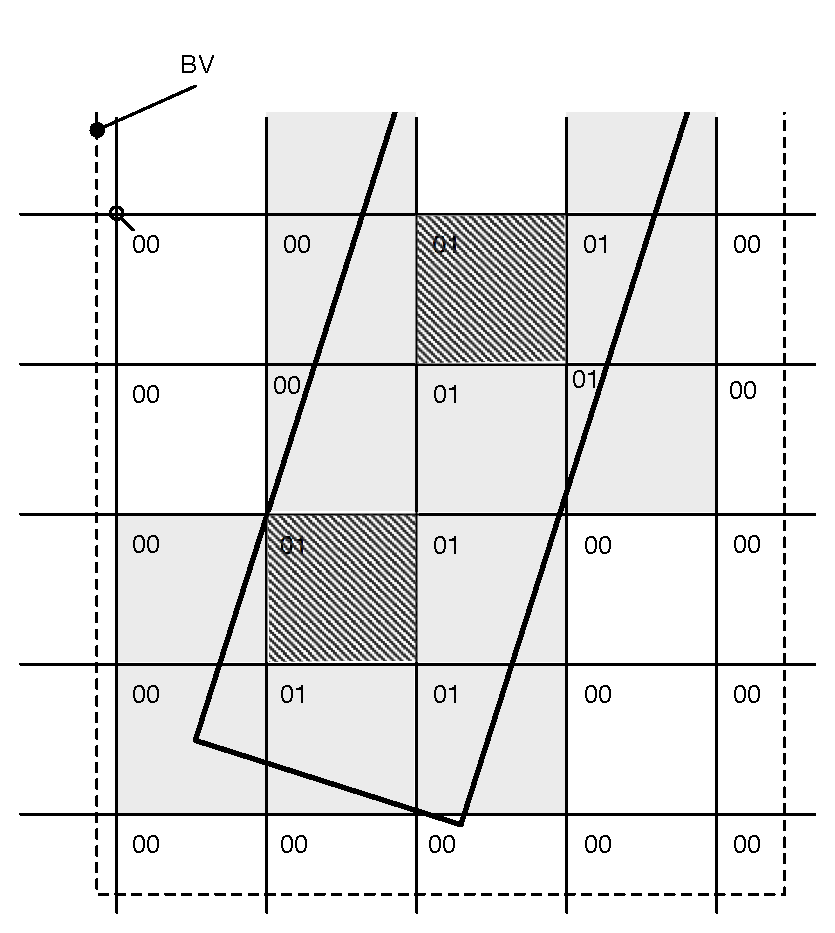
\includegraphics[width=7cm,clip]{compo_BVH.eps}
\end{center}
\end{minipage}
\begin{minipage}{0.45\hsize}
\begin{center}
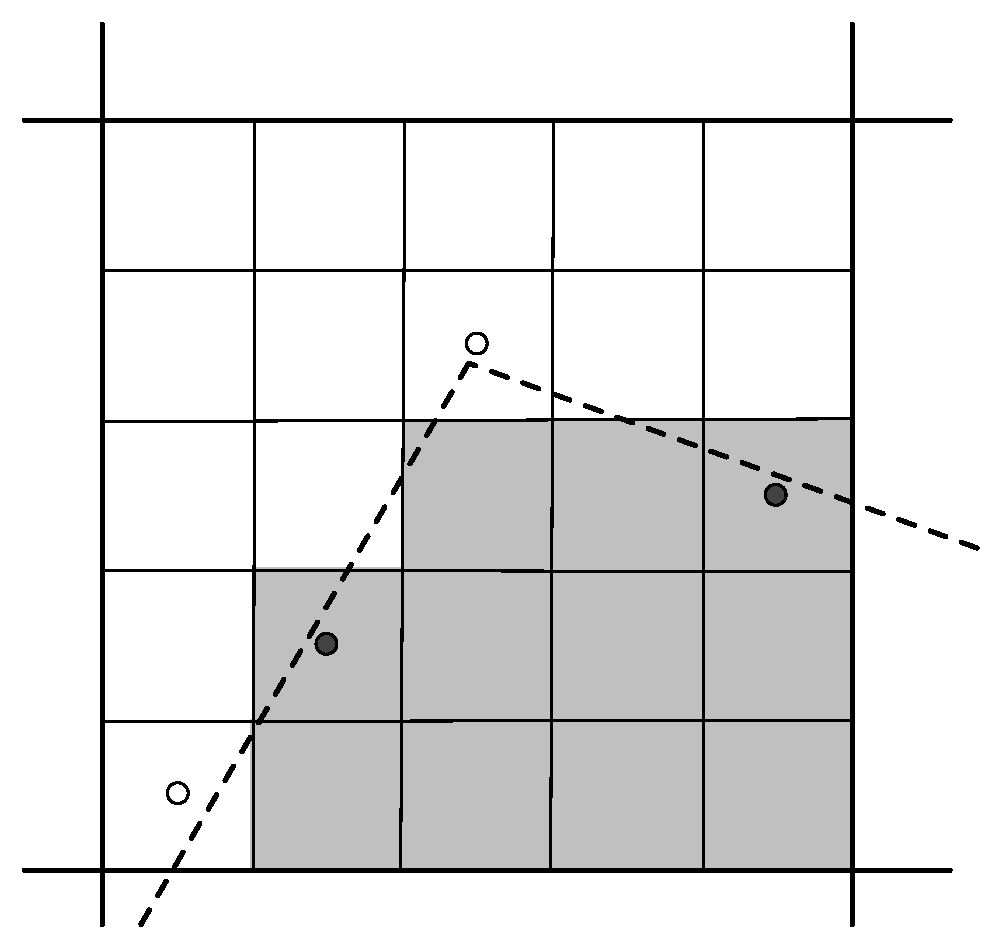
\includegraphics[width=6cm,clip]{subsampling.eps}
\end{center}
\end{minipage}
\caption{占有率の計算は,ノードの暫定的な体積率から,サブサンプリングする要素を特定する.グレー部分がサブサンプリング対象で,ハッチング部分は完全に内部にあるセル.サブサンプリングでは,セルセンタ位置でサンプリングを行い,占有率を計算する.右図は二次元の場合でn=5,11/25の占有率となる.}
\label{fig:sub-sampling}
\end{figure}

%
\paragraph{アフィン変換}
コンポーネントの形状は,空間内の任意の位置に存在する.また,その配置は格子に沿うとは限らない.
そこで内外判定を簡単にするため,コンポーネントの法線$\overrightarrow{n}$と座標の$z$軸方向の単位ベクトルが一致するように,コンポーネントBVの矩形領域をアフィン変換し,マッピングする.
さらに,点$O_R$と原点を一致させるように平行移動する.
この座標変換により,コンポーネントのBVは\textbf{図\ref{fig:compo transform}}のようになる.

\begin{figure}[htdp]
\begin{minipage}{0.45\hsize}
\begin{center}
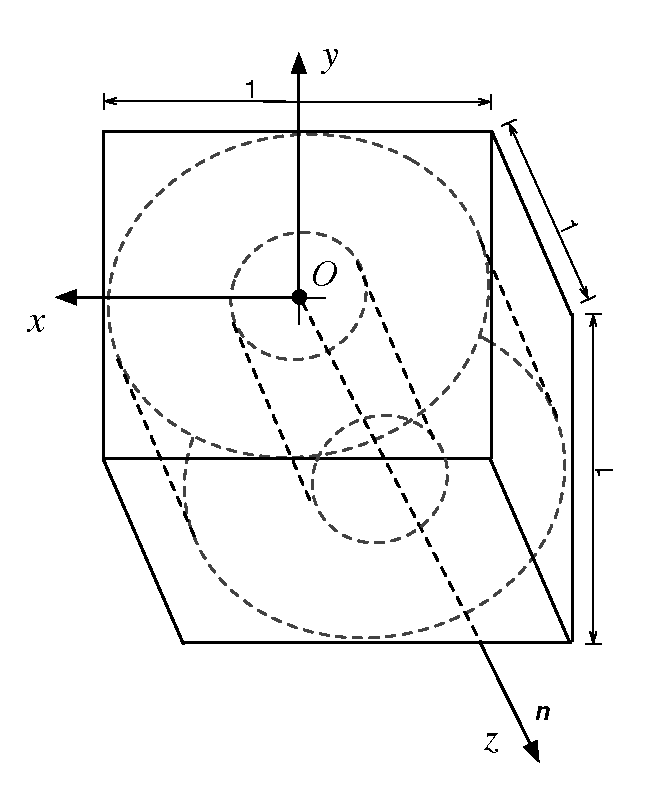
\includegraphics[width=6.5cm,clip]{compo_trnsfm.eps}
\end{center}
\end{minipage}
\begin{minipage}{0.5\hsize}
\begin{center}
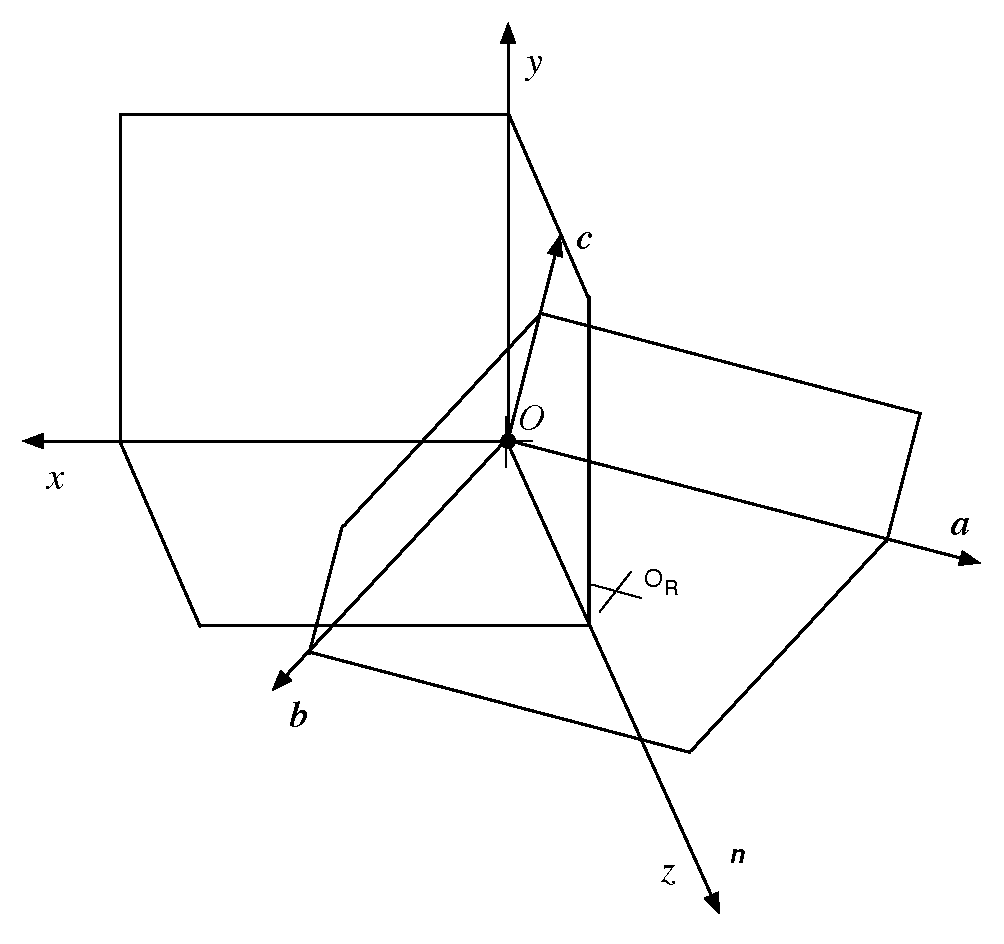
\includegraphics[width=8cm,clip]{Transform.eps}
\end{center}
\end{minipage}
\caption{コンポーネントのアフィン変換.任意の配置から,単位立方体へマッピングする.局所基底の取り方は,流出方向が$\bm c$となるようにする.}
\label{fig:compo transform}
\end{figure}

\begin{enumerate}
\item Appendixに示す\hyperlink{tgt:affin}{アフィン変換}の準備のために,\textbf{図\ref{fig:geometry_info}}の局所座標の基点を原点に平行移動し,\textbf{図\ref{fig:compo transform}}の右図のように配置する.
コンポーネントの局所座標の取り方は,\textbf{図\ref{fig:geometry_info}}の$(\bm a,\, \bm b,\, \bm c)$のように取る.
まず,法線ベクトル$\bm c$を流出方向にとり,それと直交する補助ベクトル$\bm a,\, \bm b$を右手系になるように取る.
\item このとき,変換行列の各成分は\textbf{式(\ref{eq:coef-before})}となる.
\item $O_R$を原点に重ねるように平行移動し,\textbf{図\ref{fig:compo transform}}の左図になるようにする.
\end{enumerate}


%
\paragraph{内外判定}
内外判定は,矩形領域の場合には単位立方体内にあるかどうかの判定,ファンの場合には$xy$平面でブレード部にあるかどうかを見て,奥行き方向の範囲に収まっているかで判定する.

%
\paragraph{サブサンプリング}
対象となるセルに対して,$n^3$のサブセルを想定し,サブセルのセルセンター位置でサンプリングを実行する.
オリジナルの空間座標でサンプリング点を求め,それを座標変換して内外判定を行う.

\pagebreak
%
\section{Immersed Boundary}
\label{sec:Immersed Boundary Method}
Immersed Boundary Methodの中でDirect Forcingとして知られる方法\cite{Yusof:97:CTR-ARB}を実装する.これは,指定した速度成分を指定セルに与える境界条件である.Navier-Stokes方程式に強制力を表す外力項${F_{DF}}_{i}$を導入する.

\begin{equation}
\begin{array}{l}
\displaystyle{
{\frac{\partial u_{i}}{\partial t}}^{n+1} 
\, =\, H_{i}
- {\frac{\partial p}{\partial x_{i}}}^{n+1} + {F_{DF}}_{i}
}\\
\displaystyle{
H_{i} \,=\, - \frac{\partial}{\partial x_{j}} \left({ u_{i} u_{j} }\right)
+ \frac{1}{Re} \frac{\partial}{\partial x_{j}} 
\left({ \frac{\partial u_{i}}{\partial x_{j}} + \frac{\partial u_{j}}{\partial x_{i}} }\right) 
}
\end{array}
\label{NS_IB ND}
\end{equation}

${F_{DF}}_{i}$は${u_{i}}^{n+1}=u_{i}^{T}$を満足するように与えられる,つまり,

\begin{equation}
{F_{DF}}_{i} \,=\, - H_{i} 
+ {\frac{\partial p}{\partial x_{i}}}^{n+1}
+ \frac{u_{i}^{T} - u_{i}^{n}}{\Delta t}
\label{Direct forcing term}
\end{equation}

これは,速度ベクトルに,次ステップで指定したい速度${u_{i}}^{T}$を代入することで実装できる.
この外力の導入により,強制した部分の連続の式にソース項$S_{DF}$が同時に導入される.したがって,Poisson反復の収束判断には速度の発散値の指標を用いない方が良い.ただし,$S_{DF}$の値は経験上,収束閾値よりも大きいが小さな値にとどまることが多い.

\begin{equation}
{\frac{\partial u_{i}}{\partial x_{i}}}^{n+1} \, =\, S_{DF}
\label{Cont_IB_src ND}
\end{equation}

Fractional Step法による解法の手順を示すと,
\begin{enumerate}
\item Pseudo vector
\begin{equation}
\begin{array}{ll}
\displaystyle{ \frac{{u_{i}}^{*} - {u_{i}}^{n}}{\Delta t} \,=\, {H_{i}}^{n} } & (1st\,Order)\\
\displaystyle{ \frac{{u_{i}}^{*} - {u_{i}}^{n}}{\Delta t} \,=\, \frac{3}{2}{H_{i}}^{n} - {H_{i}}^{n-1} } & (2nd\,Order)
\end{array}
\label{DF pesudo}
\end{equation}

\item Poisson
\begin{equation}
\frac{\partial}{\partial x_{i}} {\frac{\partial P}{\partial x_{i}}}^{n+1} \,=\, 
\frac{1}{\Delta t} {\frac{\partial u_{i}}{\partial x_{i}}}^{*}
\label{DF Poisson}
\end{equation}

\item Projection
\begin{equation}
\frac{{u_{i}}^{**} - {u_{i}}^{*}}{\Delta t} \,=\, - \frac{\partial}{\partial x_{i}} {\frac{\partial P}{\partial x_{i}}}^{n+1}
\label{DF Projection}
\end{equation}

\item Forcing
\begin{equation}
\begin{array}{l}
\displaystyle{ \frac{{u_{i}}^{n+1} - {u_{i}}^{**}}{\Delta t} \,=\, {F_{DF}}_{i} }\\
\displaystyle{ {F_{DF}}_{i} \,=\, \frac{{u_{i}}^{T} - {u_{i}}^{**}}{\Delta t} }
\end{array}
\label{DF forcing}
\end{equation}
このステップでは,指定領域内部の速度定義点に所望の速度${u_{i}}^{T}$を強制する.

\end{enumerate}

%
\begin{comment}
\section{sec:開口率モデル}
開口率モデルでは,指定されたセルの表面の開口面積を指定する.単独,あるいは多孔質体モデルと組み合わせても利用可能である.
\textbf{式(\ref{FVM:NS})}と\textbf{式(\ref{FVM discrete:NS})}を参考に,対流項のみを有限体積的に考える.セル幅を$h$とすると,

\begin{equation}
\frac{\partial \boldmath{u}}{\partial t} 
\,=\, 
- \frac{1}{V} \sum\limits_{i} { \boldmath{uu}_{i} \cdot \boldmath{n}_{i} \hspace{0.3em} \Delta s_{i} }
\,=\,
- \frac{1}{V} \sum\limits_{i} { \boldmath{uu}_{i} \cdot \boldmath{n}_{i} \hspace{0.3em} A_{i}\, h^{2}}
\label{Area Fraction NS}
\end{equation}

ここで$A_{i}$はセルのi番目のフェイスの開口率である.開口率の定義は,\textbf{図\ref{area def}}に示すように,流動に有効な面積をセル幅を基準にした無次元パラメータであり,二次元の場合には\textbf{式(\ref{open rate})}で定義する.

\begin{equation}
A \,=\, \frac{h_{a}}{h} \qquad [-]
\label{open rate}
\end{equation}


一旦,対流流束を計算した後,開口率が定義されている部分のみに開口率を乗じて流束を制限することにより,セル界面での閉塞効果を導入する.

\begin{figure}[htbp]
\begin{center}
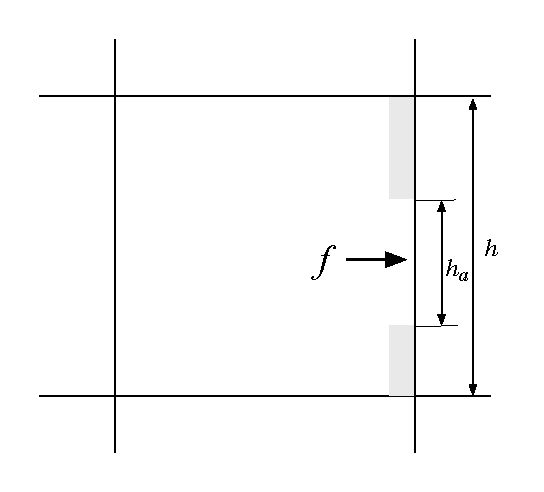
\includegraphics[width=6.5cm,clip]{AreaFraction.eps}
\end{center}
\caption{開口率の定義}
\label{area def}
\end{figure}

\end{comment}











